\documentclass[11pt,a4paper,twoside,onecolumn,openany,final,oldfontcommands]{memoir}
\usepackage{sty/FOBOS}  % FOBOS SDN style file

%%%%%%%%%%%%%%%%%%%%%%%%%%%%%%%%%%%%%%%%%%%%%%%%%%%%%%%%%%%%%%%%%%%%%%%%
%%%%%%%%%%%%%%%%%%%%%%%%%%%%%%%%%%%%%%%%%%%%%%%%%%%%%%%%%%%%%%%%%%%%%%%%
% Things you need to edit:
%   - Document name, numbering, and date; edit the newcommands below.
%   - Authors list; see authors.tex
%   - The contact information for the corresponding author; see corresponding.tex
%   - Any (additional) tex aliases you would like to include; see aliases.tex
%   - BibTex references are included using ref.bib
%   - Main body of the document
%   - Add a line to the revision history

\newcommand{\doclongname}{Science Requirements Document}
\newcommand{\docshortname}{SRD}

\newcommand{\project}{FOBOS}
\newcommand{\wbs}{TOP}
\newcommand{\doctype}{DOC}
\newcommand{\docnumber}{001}

% Pre-release versions are 0A - ZZ; Release versions should be 01-99
\newcommand{\docversion}{0A}
\newcommand{\docreleaseDate}{2020-07-08}  % Please use ISO-8601 YYYY-MM-DD format.

%%%%%%%%%%%%%%%%%%%%%%%%%%%%%%%%%%%%%%%%%%%%%%%%%%%%%%%%%%%%%%%%%%%%%%%%
%%%%%%%%%%%%%%%%%%%%%%%%%%%%%%%%%%%%%%%%%%%%%%%%%%%%%%%%%%%%%%%%%%%%%%%%

% Document Designation Number
\newcommand{\docsysnum}{{\project}.{\wbs}.{\doctype}.{\docnumber}.V{\docversion}}

%% Set footers to use document info
%% ================================
\makeoddfoot{Ruled}{\docsysnum}{}{\thepage\ / \thelastpage}
\makeevenfoot{Ruled}{\thepage\ / \thelastpage}{}{\docsysnum}

%%% Packages for TESTING
\usepackage{lipsum}
\listfiles

%% ALIASES

%\newcommand{\asic}{Application Specific Integrated Circuit}
%\newcommand{\DRC}{Design Reference Case}
%\newcommand{\keck}{W.~M.~O. Keck Observatory}
%\newcommand{\ie}{\emph{i.e.\ }}
%\newcommand{\scales}{Santa Cruz Array of Lenslets for Exoplanet Spectroscopy}
%\newcommand{\inst}{FOBOS}
%\newcommand{\sidecar}{SIDECAR}
%\newcommand{\SIDECAR}{System for Image Digitization, Enhancement, Control and Retrieval}
%\newcommand{\SWG}{Science Working Group}
%\newcommand{\tis}{Teledyne}
%\newcommand{\TIS}{Teledyne Imaging Sensors}
%\newcommand{\ucscfull}{University of California Santa Cruz}
%\newcommand{\ucsc}{UCSC}
%\newcommand{\wrt}{with respect to}

\newcommand{\farcm}{\mbox{\ensuremath{.\mkern-4mu^\prime}}}  % fractional arcminute: 0.'0
\newcommand{\farcs}{\mbox{\ensuremath{.\!\!^{\prime\prime}}}}  % fractional arcsec: 0.''0
\newcommand{\fdg}{\mbox{\ensuremath{.\!\!^\circ}}}  % fractional degree:  0.¡0
\newcommand{\arcdeg}{\ensuremath{^{\circ}}}  % degree symbol:  ¡
\newcommand{\arcmin}{\ensuremath{^{\prime}}}  % degree symbol:  ¡
\newcommand{\arcsec}{\ensuremath{^{\prime\prime}}}  % degree symbol:  ¡
\newcommand{\sun}{\ensuremath{\odot}}  % sun symbol

\newcommand{\msun}{M$_{\odot}$}
\newcommand{\Msun}{{\rm M}_{\odot}}
\newcommand{\Hz}{{\rm Hz}}
\newcommand{\erg}{{\rm erg}}
\newcommand{\yr}{{\rm yr}}
\newcommand{\cm}{{\rm cm}}
\newcommand{\kms}{{\rm km s$^{-1}$}}
\newcommand{\s}{{\rm s}}
\newcommand{\Mpc}{{\rm Mpc}}
\newcommand{\Halpha}{{H$\alpha$}}
\newcommand{\Hbeta}{{H$\beta$}}
%\newcommand{\Mgb}{{Mg$_{\rm b}$}}
\newcommand{\Mgb}{Mg{\it b}}
\newcommand{\Reff}{{R$_{e}$}}
\newcommand{\HI}{{\sc H\,i}}
\newcommand{\HII}{{\sc H\,ii}}
\newcommand{\photoz}{photo-$z$}

\newcommand{\gaia}{\textit{Gaia}}
\newcommand{\euclid}{\textit{Euclid}}




%%%% BEGIN DOCUMENT
\begin{document}
\bibliographystyle{sty/aasjournal}

%%% FRONTMATTER
\frontmatter
{\begingroup
\newlength{\drop}
\drop=0.1\textheight
\begin{flushleft}
    
\includegraphics[width=\textwidth]{figs/logo/FOBOS_LOGO_FINAL.png}

    \vspace{0.5\drop}
    \begin{Spacing}{1.5}
    {\huge \doclongname\\ (\docshortname)}
    \end{Spacing}
    \vfill

    \vfill
    {\Large
    % Authors
Kyle B.\ Westfall,\textsuperscript{1}
Kevin A.\ Bundy,\textsuperscript{1,2}
Daniel C.\ Masters,\textsuperscript{3}
Joseph N.\ Burchett,\textsuperscript{2}
V.\ Ashley Villar,\textsuperscript{4}
R.\ Michael Rich,\textsuperscript{5}
Benjamin F.\ Williams,\textsuperscript{6}
Nathan Sandford,\textsuperscript{7}
and
Yuan-Sen Ting \textsuperscript{8}

% Affiliations
\begin{small}
\textsuperscript{1}University of California Observatories;
\textsuperscript{2}University of California, Santa Cruz;
\textsuperscript{3}IPAC, California Institute of Technology;
\textsuperscript{4}Columbia University;
\textsuperscript{5}University of California, Los Angeles;
\textsuperscript{6}University of Washington;
\textsuperscript{7}University of California, Berkeley
\textsuperscript{8}The Australian National University
\end{small}


    }
    \vfill

    {\LARGE \bfseries \docsysnum} \\
    \docreleaseDate{} \\
    \thelastpage\ pages

\end{flushleft}
\vspace*{0.5\drop}
\endgroup}

\thispagestyle{empty}  % Title page has no page number shown.

\clearpage
\setupmaintoc
\tableofcontents 

\clearpage
\listoffigures

\clearpage
\listoftables

%: PREFACE
\chapter{Corresponding Author}
%
\begin{table}[htp]
\begin{center}
\begin{tabular}{l}
    Kyle B.\ Westfall, \emph{FOBOS Project Scientist} \\
    University of California Observatories \\
    University of California, Santa Cruz \\
    1156 High Street\\
    Santa Cruz, CA 95064 USA \\
    \\
    +1-831-459-4362 \\ 
    \\
    {\ttfamily westfall@ucolick.org}
\end{tabular}
\end{center}
\end{table}%



%%%%%%%%%%%%%%%%%%%%%%%%%%%%%%%%%%%%%%%%%%%%%%%%%%%%%%%%%%%%%%%%%%%%%%%%
%%%%%%%%%%%%%%%%%%%%%%%%%%%%%%%%%%%%%%%%%%%%%%%%%%%%%%%%%%%%%%%%%%%%%%%%
% The rest of the document editing begins here

%-----------------------------------------------------------------------
% Executive Summary
\chapter{Executive Summary}

\edit{This is the FOBOS science-requirements document.}

%-----------------------------------------------------------------------


%-----------------------------------------------------------------------
% Main document body
\mainmatter

\chapter{Introduction}

\section{Motivation}

Led by the Vera C.~Rubin Observatory Legacy Survey of Space and Time (LSST)\footnote{For the first ten years of operation, Vera C.~Rubin Observatory will perform the Rubin Observatory Legacy Survey of Space and Time (LSST). The National Science Foundation (NSF) and the US Department of Energy (DOE) are joint partners in the Rubin Observatory Project and Operations.} and NASA-supported missions like \euclid\footnote{\euclid\ is led by the European Space Agency with significant NASA involvement and will launch in 2022. Its primary mission is a 15,000 deg$^2$ imaging and grism survey in optical and near-IR wavebands.} and the Nancy Grace Roman Space Telescope,\footnote{The Nancy Grace Roman Space Telescope is expected to launch in the mid 2020's.} astronomy is entering a new era of unprecedented deep-imaging campaigns that will survey huge volumes of the universe. From the emergence of the earliest galaxies from a baryonic ``primordial soup,'' through the epoch of cosmic expansion, to the evolved structure of present-day galaxies in our own Local Group and the promise of time-domain discoveries, images from these surveys will provide unprecedented insights into key epochs of cosmic history. As such, these surveys were ranked as top priorities in the Astro2010 decadal survey, resulting in a significant investment of U.S.\ funding agencies in their success.

The need for spectroscopic follow-up of these vast imaging campaigns is obvious.  Indeed, the success of the Sloan Digital Sky Survey (SDSS) and anticipated for the Dark Energy Spectroscopic Instrument (DESI) has made clear the scientific value of coupling panoramic imaging with intensive spectroscopic follow-up, both in terms of new discoveries and in dramatically improving our statistical understanding of the cosmos.  However, at the end of the next decade, these facilities will deliver photometric data across vast areas at a depth that is 1,000 times below SDSS imaging, and \textit{no current U.S.~facility is capable of obtaining spectroscopic follow-up at these depths} at the level required to capitalize on the $\approx$\$4B U.S.\ investment in these projects. In fact, an SDSS-like spectroscopic study of 1 million galaxies at LSST depths would require 300 years of observing on the largest telescopes with current instrumentation!

It has long been recognized that a new spectroscopic facility is needed to meet the challenge presented by this era of deep, panchromatic imaging. For example, the National Research Council's 2015 report, ``Optimizing the U.S. Ground-Based Optical and Infrared Astronomy System'' \citep{NAP21722} states:
%
\noindent\begin{center}\mbox{\parbox{0.95\linewidth}{
%
The National Science Foundation should support the development of a wide-field, highly multiplexed spectroscopic capability on a medium- or large-aperture telescope in the Southern Hemisphere to enable a wide variety of science, including follow-up spectroscopy of Large Synoptic Survey Telescope\footnote{Now renamed to be the Rubin Observatory Legacy Survey of Space and Time, as noted previously.} targets. Examples of enabled science are studies of cosmology, galaxy evolution, quasars, and the Milky Way.
%
}}\end{center}
%
Additionally, workshops organized by the National Optical Astronomy Observatory (NOAO) in 2013 and 2016, the latter at request of the NSF, reported specific spectroscopic needs for follow-up of LSST sources in all science areas.  In particular, the 2016 report notes that a critical resource in need of prompt development is to ``Develop or obtain access to a highly multiplexed, wide-field optical multi-object spectroscopic capability on an 8m-class telescope.''

Particularly for the U.~S.\ astronomical community, the twin 10m telescopes of the W.~M.~Keck Observatory (WMKO) represent a compelling avenue to meet this need.  While its location in the northern hemisphere is somewhat limiting, more than 60\% of the LSST footprint and three of its deep-drilling fields (COSMOS, XMM-LSS, and E-CDFS) are within the WMKO visibility window.  \edit{More on overlap with Roman, \euclid, $+$.}  Additionally, WMKO provides the only \textit{existing} telescope infrastructure with a 10-m aperture, and, given its site and mirror coatings, is uniquely sensitive toward the atmospheric limit in the UV.  The limited multiplex capacity and sensitivity (compared to more modern equivalents) of its current instruments for optical spectroscopy motivates the need for a much more capable instrument.  Moreover, it is significantly more cost effective to invest in a new instrument for an existing facility than it would be to build an entirely new 10m-telescope$+$spectroscopic facility in the southern hemisphere.

Supporting spectroscopic follow-up of large-scale survey missions is already in lockstep with WMKO's strategic goals.  Specifically, the 2016 WMKO Scientific Strategic Plan (SSP) highlights that WMKO ``works best by undertaking sensitive observations of sources found by surveys or other facilities.''  In fact, the 2016 WMKO Scientific Strategic Plan recommended pursuit of ``highly multiplexed, highly sensitive spectroscopy'' as its top-priority design study.  Although largely cast as upgrades to existing instruments (e.g., adding a second DEIMOS channel), Appendix II of the SSP specifically notes recent improvements in the sophistication of fiber-based instruments that are ``improving throughput, increasing sky subtraction accuracy, and increasing the density of fibers that can be stacked along the fiber pseudo-slit. All of these trends deepen the limiting magnitude attainable with fibers, as well as the number of objects than can be surveyed.''

These considerations have lead to our concept for the \textbf{Fiber-Optic Broadband Optical Spectrograph, FOBOS,} timed to deploy on WMKO's Keck II Telescope in 2028, just as various panoramic deep-imaging surveys begin reaching their target depths.  FOBOS emphasizes flexible and quickly configurable focal-plane sampling with high multiplex, UV sensitivity, and a stable spectral format that supports ultra-deep integrations of $\gtrsim$50 hours, thereby building from and expanding on traditional strengths of WMKO observations.

% Based on these recommendations, we propose the FOBOS instrument coupled with a suite of data-driven tools to address the spectroscopic requirements of LSST and other photometric surveys at a final cost 20 times less than a new Southern Hemisphere facility. Located in Hawaii, FOBOS can access more than 70\% of the LSST footprint, more than adequate for building powerful spectroscopic training sets.


% Multiple observing modes are possible, including PI-led programs, survey-level campaigns, and queue-scheduled observations.  In combination, these modes will enhance overall science return by enabling human interaction while maximizing efficiency.  FOBOS's conceptual design has been driven by four ``design-reference'' science programs centered on studies of the nature of Dark Energy (\S \ref{sec:cosmology}), the formation of galaxies (\S \ref{sec:galaxies}), the physical properties of kilonovae (\S \ref{sec:kilonovae}), and the assembly history of the Andromeda Galaxy system (\S \ref{sec:localgroup}).  Each program would advance the scientific frontier anticipated at the time of FOBOS commissioning in 2028, both in terms of direct interpretation of the observations themselves and their use in machine-learning methods that can train and deliver physical inferences for the upcoming trove of photometric samples (\S \ref{sec:ML}).

% The instrument will simultaneously collect spectra from 1800 fibers distributed among single apertures and/or integral-field units (IFUs) across a 20$^\prime$ field.  FOBOS provides deep sensitivity, with $\gtrsim$30\% instrument throughput from 0.31--1.0 $\mu$m, and a spectral resolution of $R \sim 3500$ delivered by three, bench-mounted 4-channel spectrographs (see Table~\ref{tab:specsummary}).  FOBOS will be a premier facility for follow-up of rare, faint, and transient sources; it will map galaxies and their environments from scales of pc to tens of Mpc; and it will excel at providing the \emph{deep-drilling} spectroscopic training sets required to extract maximum information from the upcoming wealth of wide-field photometry. Its innovative and flexible target-allocation system and multiplexed IFU modes provide unique capabilities for realizing major progress on fundamental goals in cosmology, galaxy formation, transient characterization, and Local-Group archaeology. FOBOS provides direct benefits to the U.S.\ community (beyond traditional Keck users) through community-led, public, key-science programs (\S \ref{sec:community}). Additional ``open-access'' to a proposed $\sim$100,000 fiber-hours per year (equivalent to 160 DEIMOS and 270 LRIS-B nights per year) will support PI-led programs from U.S.\ astronomers. Raw, reduced, and high-level data products (e.g., redshifts, line fluxes, continuum fits) will be publicly released for \emph{all} FOBOS observations and served via the Keck Observatory Archive on a science-ready platform (see Data Management Plan).  Finally, signaling its support of broad community engagement, WMKO has agreed to provide immediate open-access to all Keck instruments for 30 nights from 2021--2024, to be allocated by a national time allocation committee (TAC) should this proposal be successful.



% High-multiplex and deep spectroscopic follow-up of upcoming panoramic deep-imaging surveys like LSST, Euclid, and WFIRST is a widely recognized and increasingly urgent necessity. No current or planned facility at a U.S.~observatory meets the sensitivity, multiplex, and rapid-response time needed to exploit these future datasets. FOBOS, the Fiber-Optic Broadband Optical Spectrograph, is a near-term fiber-based facility that addresses these spectroscopic needs by optimizing depth over area and exploiting the aperture advantage of the existing 10m Keck II Telescope. The result is an instrument with a uniquely blue-sensitive wavelength range (0.31--1.0 $\mu$m) at $R \sim 3500$, high-multiplex (1800 fibers), and a factor 1.7 greater survey speed and order-of-magnitude greater sampling density than Subaru's Prime Focus Spectrograph (PFS). In the era of panoramic deep imaging, FOBOS will excel at building the deep, spectroscopic reference data sets needed to interpret vast imaging data. At the same time, its flexible focal plane, including a mode with 25 deployable integral-field units (IFUs) across a 20 arcmin diameter field, enables an expansive range of scientific investigations. Its key programmatic areas include (1) nested stellar-parameter training sets that enable studies of the Milky Way and M31 halo sub-structure, as well as local group dwarf galaxies, (2) a comprehensive picture of galaxy formation thanks to detailed mapping of the baryonic environment at $z \sim 2$ and statistical linking of evolving populations to the present day, and (3) dramatic enhancements in cosmological constraints via precise photometric redshifts and determined redshift distributions.  In combination with Keck I instrumentation, FOBOS also provides instant access to medium-resolution spectroscopy for transient sources with full coverage from the UV to the K-band.

% With its high multiplex and Keck's large aperture, FOBOS will enable significant progress in multiple science areas by
% providing much-needed large and deep spectroscopic samples.  These unprecedented data sets will be scientific gold
% mines for the U.S.~community in their own right, but when combined with novel observations from forthcoming facilities,
% transformational advances are possible.  These include 1) charting the assembly history of the Milky Way, M31, and
% Local Group dwarf galaxies by combining deep FOBOS spectroscopy with wide spectroscopic campaigns (e.g., DESI
% Bright-Time Survey and SDSS-V Milky Way Mapper), GAIA data, and panoramic imaging from LSST, Euclid, and WFIRST; 2)
% mapping the baryonic ecosystem at $z \sim 2$--3 and linking it to evolving populations at lower redshifts by training
% photometric diagnostics that transfer detailed spectroscopic knowledge to billion-plus galaxy samples provided by
% future all sky surveys; 3) dramatically enhancing cosmological probes using panoramic deep imaging and
% cross-correlation techniques with Stage-IV CMB observations thanks to precise calibration of photometric redshifts and
% redshift distributions.

% FOBOS addresses these goals by achieving high multiplex while optimizing for sensitivity over area.  Future imaging data will routinely reach $i_{\rm AB} = 25$, yielding target densities of 42 arcmin$^{-2}$.  FOBOS achieves a single-pass on-sky sampling density of 6 arcmin$^{-2}$ on average, and close packing would allow a maximum target density of $\sim$30 arcmin$^{-2}$.  These capabilities allow FOBOS to collect large samples of very faint sources with highly efficient observing strategies. 

% \paragraph{FOBOS's Key Science Questions:}

% \begin{enumerate} 
% \item What is the nature of the assembly histories of the Milky Way, M31, and Local Group dwarfs?  {\em (Section \ref{sec:LocalGroup})}
% \item What are the key processes driving the late-time evolution of galaxies from $z\sim 1$ to the present day? {\em (Section \ref{sec:galaxies})}
% \item How is the baryonic environment at $z \sim 2$--3 influenced by forming galaxies and how does it drive their formation? {\em (Section \ref{sec:galaxies})}
% \item What is the nature of Dark Energy and the growth of cosmic structure at high redshift? {\em (Section \ref{sec:cosmology})}
% \end{enumerate}

\section{Scope}

As a facility-class instrument, FOBOS will be used to pursue a wide range of scientific goals.  The purpose of this document is to encapsulate the breadth and depth of these goals in a way that flows down to the instrument-defining technical requirements.  This document enumerates and provides the justification for all instrument requirements, which are further developed and refined in the Design Reference Document (DRD; FOBOS.TOP.DOC.002; \edit{include link}).

During its Conceptual Design Phase (CoDP), FOBOS science requirements have been developed following two paths: (1) We capture the core science that FOBOS \textit{must} enable via a series of  ``design-reference'' programs.  These programs represent the most compelling uses of FOBOS in its first few years on sky, addressing key science questions that we expect to be particularly timely.  We refer to these as \textbf{Key Programs} and discuss them in terms of observations that ``will'' be done; however, we emphasize that, as of the current release of this document (\docsysnum), the execution of these programs is not guaranteed.  (2) Additional \textbf{Science Drivers} are presented that have not (yet) led to large-scale observing programs, but also represent compelling science that FOBOS \textit{must} enable.

Development of the Key Programs and Science Drivers emphasizes a full exploration of the instrument needs for any given science case.  However, from the outset, this was done within the context of the following gross expectations for the final instrument design:
%
%{\tightlists
\begin{asparaenum}
\item improves upon the current DEIMOS multiplex,
\item follows a fiber-fed, modular spectrograph design,
\item provides both single-aperture and integral-field capabilities,
\item samples the optical-to-NIR wavelength range, and
\item provides modest spectral resolution ($R\sim 3000-5000$).
\end{asparaenum}
%}

% The distinction between these two development paths is as follows: Science Drivers primarily explore FOBOS's instrument capabilities for a given observation, whereas Key Programs also explore its operational capabilities for executing a given program.  For example, a Science Driver may require that the spectral range covers the IMF-sensitive Wing-Ford band in the red (\edit{ref}), whereas a Key Program may also require that FOBOS observe this feature in $N$ galaxies over $M$ dark nights to measure the change in the IMF slope as a function of stellar mass to a precision of better than $X$ dex at a redshift of $z\lesssim 0.1$.

% Probably need a better name for "science" requirements.

Let's try this again.

Requirements derived from the Key Programs and Science Drivers are divided into program requirements and science requirements:  \textbf{Program requirements} lead to instrument requirements that enable program success; e.g., ``To measure a change in the slope of the initial mass function (IMF) of $X$ dex per ${\rm d}(\log\mathcal{M}_\ast)$ or larger, the equivalent width of the Wing-Ford band must be measured to better than $Y$ dex for $N$ galaxies evenly distributed over a mass range of $\mathcal{M}_1 < \mathcal{M}_\ast < \mathcal{M}_2$.''  \textbf{Science requirements} lead to instrument requirements that enable a given measurement; e.g., ``The spectral range must include the Wing-Ford band (989 nm $< \lambda <$ 995 nm) for galaxies at $z \lesssim 0.1$.''  \edit{This isn't a great example because we don't actually meet that requirement.}  A useful distinction is that program requirements can flow down to one or more science requirements, but not vice versa. Program and science requirements are signified by \textbf{P} (e.g., \textbf{P 2.1}) and \textbf{S}, respectively.

This document consolidates the program and science requirements into a series of \textbf{instrument requirements} and \textbf{data requirements}.  Here, we distinguish between requirements that are primarily driven by the instrument hardware from those primarily driven by the software related to the data-management systems (DMS; Section \edit{..}).  \edit{for the purposes of this document, is it okay to consider requirements on the operational software to be ``instrument requirements?''}  For example, following from the example above, a relevant instrument requirement would be: ``The red spectral limit must be $\geq$ 1.1 $\mu$m.''  A relevant data requirement would be: ``Systematic errors in the equivalent width of the Wing-Ford band introduced by sky subtraction and flux calibration must not be larger than 10\% of the Poisson error due to photon shot noise.''  Importantly, there is an obvious interplay between the hardware and software requirements that will evolve as the limitations of each are explored. Instrument and data requirements are signified by an \textbf{R} and \textbf{D}, respectively.

Data requirements do not, as of this release, differentiate between requirements most relevant to the data-\textit{reduction} pipeline (the DMS \textit{Accountant}) versus those most relevant to the data-\textit{analysis} pipeline (the DMS \textit{Alchemist}).  Data requirements drawn from the Key Programs will provide both flavors of data requirements; however, Science Drivers may not lead to requirements for the data-analysis pipeline.  That is, although the FOBOS project aims to enable pipeline-produced high-level data products for \textit{all} FOBOS data, the project-led development of the data-analysis software will be driven by the needs of the Key Programs, at least initially.

Each of the instrument (\textbf{R}) and data (\textbf{D}) requirements point to one or more program (\textbf{P}) and/or science (\textbf{S}) requirements that it satisfies.  Summary tables provide a mapping from each instrument/data requirement to all associated program/science requirements (Tables \edit{x}) and vice versa (Table \edit{y}); each program/science requirement must lead to at least one instrument/data requirement.

% The ability to address these questions depends both on the FOBOS instrument design and the design of possible observing programs to be carried out within each science area.  This Science Requirements Document seeks to outline possible key science programs whose goals can flow down to specific instrument requirements.

\subsection{Particulars}

\edit{Pulled from the MaNGA SRD but seems relevant as is.} In discussing the science requirements, we would also like to separate `precision' from `accuracy'. All of our quantitative requirements focus on measurement precision, which includes only uncertainty propagated from raw measurement uncertainties under a specific set of model assumptions. They do not include systematic uncertainty due to incorrect model assumptions. Because there could be a large number of different model assumptions and the truth may be even beyond current knowledge, it is often a nearly impossible task to assess how accurate a physical property can be measured to its true value. Nonetheless, that is the ultimate goal of this whole enterprise. By limiting the measurement uncertainty and measuring same physical property from different methodologies, we can gain important insight about the accuracy and fidelity of the measurement. Here, we only consider measurement precision in our science requirements and do not discuss accuracy.

\edit{This needs to be edited.}
Throughout this document, we adopt a consistent signal-to-noise (S/N) definition for the stellar continuum, which is the median S/N per pixel in the logarithmic wavelength grid with $\Delta \log \lambda = 10^{-4}$ across the SDSS r-band (the linear pixel size is approximately 1.4\AA). This can be directly measured from the raw fiber spectrum and we have historical BOSS data to link this S/N to surface brightness on the sky. This allows us to estimate the S/N we can obtain in our target galaxy to check if they can meet the science requirements.

\section{Outline}

\edit{to be written}
In what follows, we collect the high-level science requirements for each of the key science questions in Section~\ref{sec:key_science} and present the flow-down into underlying requirements in terms of direct observables (Section~\ref{sec:key_observables}), the program definition (Section~\ref{sec:programs}), spectro-photometric calibration (Section~\ref{sec:spectrophotometry}), guiding and PSF metrology (Section~\ref{sec:guiding}), data reduction (Section~\ref{sec:data_reduction_pipeline}), the FOBOS data products (Section~\ref{sec:data_products}).


\newpage

\chapter{Key Programs}

\section{FOBOS Key Science}

\edit{Below is directly from the MSIP and needs to be edited.}

FOBOS will be a facility-class instrument at Keck, emphasizing flexible and quickly configurable focal-plane sampling, UV sensitivity, and a stable spectral format that supports ultra-deep integrations of $\gtrsim$50 hours.  Multiple observing modes are possible, including PI-led programs, survey-level campaigns, and queue-scheduled observations.  In combination, these modes will enhance overall science return by enabling human interaction while maximizing efficiency.  FOBOS's conceptual design has been driven by four ``design-reference'' science programs centered on studies of the nature of Dark Energy (\S \ref{sec:cosmology}), the formation of galaxies (\S \ref{sec:galaxies}), the physical properties of kilonovae (\S \ref{sec:kilonovae}), and the assembly history of the Andromeda Galaxy system (\S \ref{sec:localgroup}).  Each program would advance the scientific frontier anticipated at the time of FOBOS commissioning in 2028, both in terms of direct interpretation of the observations themselves and their use in machine-learning methods that can train and deliver physical inferences for the upcoming trove of photometric samples (\S \ref{sec:ML}).

To illustrate FOBOS's scientific potential, we present the science drivers and observing strategies for these design-reference programs.  Table \ref{tab:progreq} summarizes the details of each program and illustrates FOBOS's ability to interleave multiple programs with disparate scientific goals (\S \ref{sec:addsci}).  The final definition of FOBOS's design-reference programs, including detailed sample designs, scientific deliverables, and time requests, will be developed in the next phase through a community-wide competition organized jointly with NSF's NOIRLab (formerly NOAO) and WMKO.

\section{Photometric-redshift training for Dark Energy surveys}
\label{sec:photozs}

Stage-IV cosmology missions --- like the Vera C.~Rubin Observatory Legacy Survey of Space and Time (LSST), the ESA/NASA \euclid\ mission, and the NASA-led Nancy Grace Roman Space Telescope (Roman) --- will obtain multi-band imaging data with unprecedented depth and survey area in the coming decades.  Current survey baselines for LSST will provide \textit{ugrizy} optical imaging of $\sim$18,000~deg$^{2}$ with a detection limit 1,000 fainter than the Sloan Digital Sky Survey (SDSS), complemented by deep near-IR imaging by Roman for an overlapping $\sim$2000~deg$^{2}$.  Measurements drawn from these data of galaxy positions and gravitational shear as a function of distance over vast cosmic volumes will be used to delineate cosmic expansion and the growth of large-scale structure. Critically, the distances used for these measurements must be estimated by photometric redshifts (photo-$z$s), given the infeasibility of obtaining spectroscopic redshifts (spec-$z$s) for the expected magnitude distribution of the billions of sources imaged by these surveys (see Figure \ref{fig:cosmos_magdist}).  This reliance on photo-$z$s has led to significant effort devoted to understanding their influence on the derived cosmological parameters \citep{huterer06, hearin10, newman15, LSSTDESCSRD}.  The consensus of these studies is that improving galaxy photo-$z$ estimates represents one of the most significant gains to be made in the precision of the cosmological parameters.

Limiting uncertainties in photo-$z$ estimates involves improving photo-$z$ \textbf{training} and \textbf{calibration} \citep{newman15}.  Training focuses on improving photo-$z$s by, e.g., ensuring that the underlying spectroscopic redshifts used to establish the relationship between galaxy color and redshift sample the relevant parameter space \citep{masters15, hemmati18}.  Photo-$z$ calibration involves quantification of the accuracy and precision with which photo-$z$s map to spec-$z$s for \textit{all} galaxies used to measure dark-energy parameters of interest.  Both pursuits are critical to improving the constraining power of and minimizing the biases in the resulting cosmological parameters \citep{LSSTDESCSRD}.

A series of well-formulated observing programs have been developed that address photo-$z$ training and calibration, as summarized in a series of Astro2020 white papers \citep{newman19, hlovek19, mandelbaum19}.  However, each of these programs involve significant investment and may require deployment of new instrumentation.  In particular, \citet{newman15, newman19} outline an observing program that improves photo-$z$ training via spectroscopy of thousands of galaxies at very faint magnitudes ($i_{\rm AB} \lesssim 25.3$).  The combination of sample size and magnitude distribution make this program extremely difficult, if not impossible, with current instrumentation.  Although significant efforts \textit{are} underway to fill in underpopulated regions in the color-redshift mapping with targeted Keck spectroscopy to the anticipated \euclid\ depth\citep{masters19}, a larger-scale effort is needed to reach the fainter galaxies that will dominate the Rubin/Roman samples.

% LSST will provide a crucial extragalactic dataset in the late 2020s, providing deep \textit{ugrizy} optical imaging of $\sim$18,000~deg$^{2}$, while WFIRST will obtain deep near-IR imaging for $\sim$2000~deg$^{2}$, overlapping the LSST footprint. FOBOS will be well-positioned to contribute critical follow-up spectroscopy for both missions, with the ability to efficiently observe sources as far south as $-30^\circ$, comprising $\sim$60\% of the current baseline LSST footprint.

%\begin{wrapfigure}{r}{0.5\textwidth}%\small
%\vspace{-0.2cm}
\begin{figure}
\begin{center}
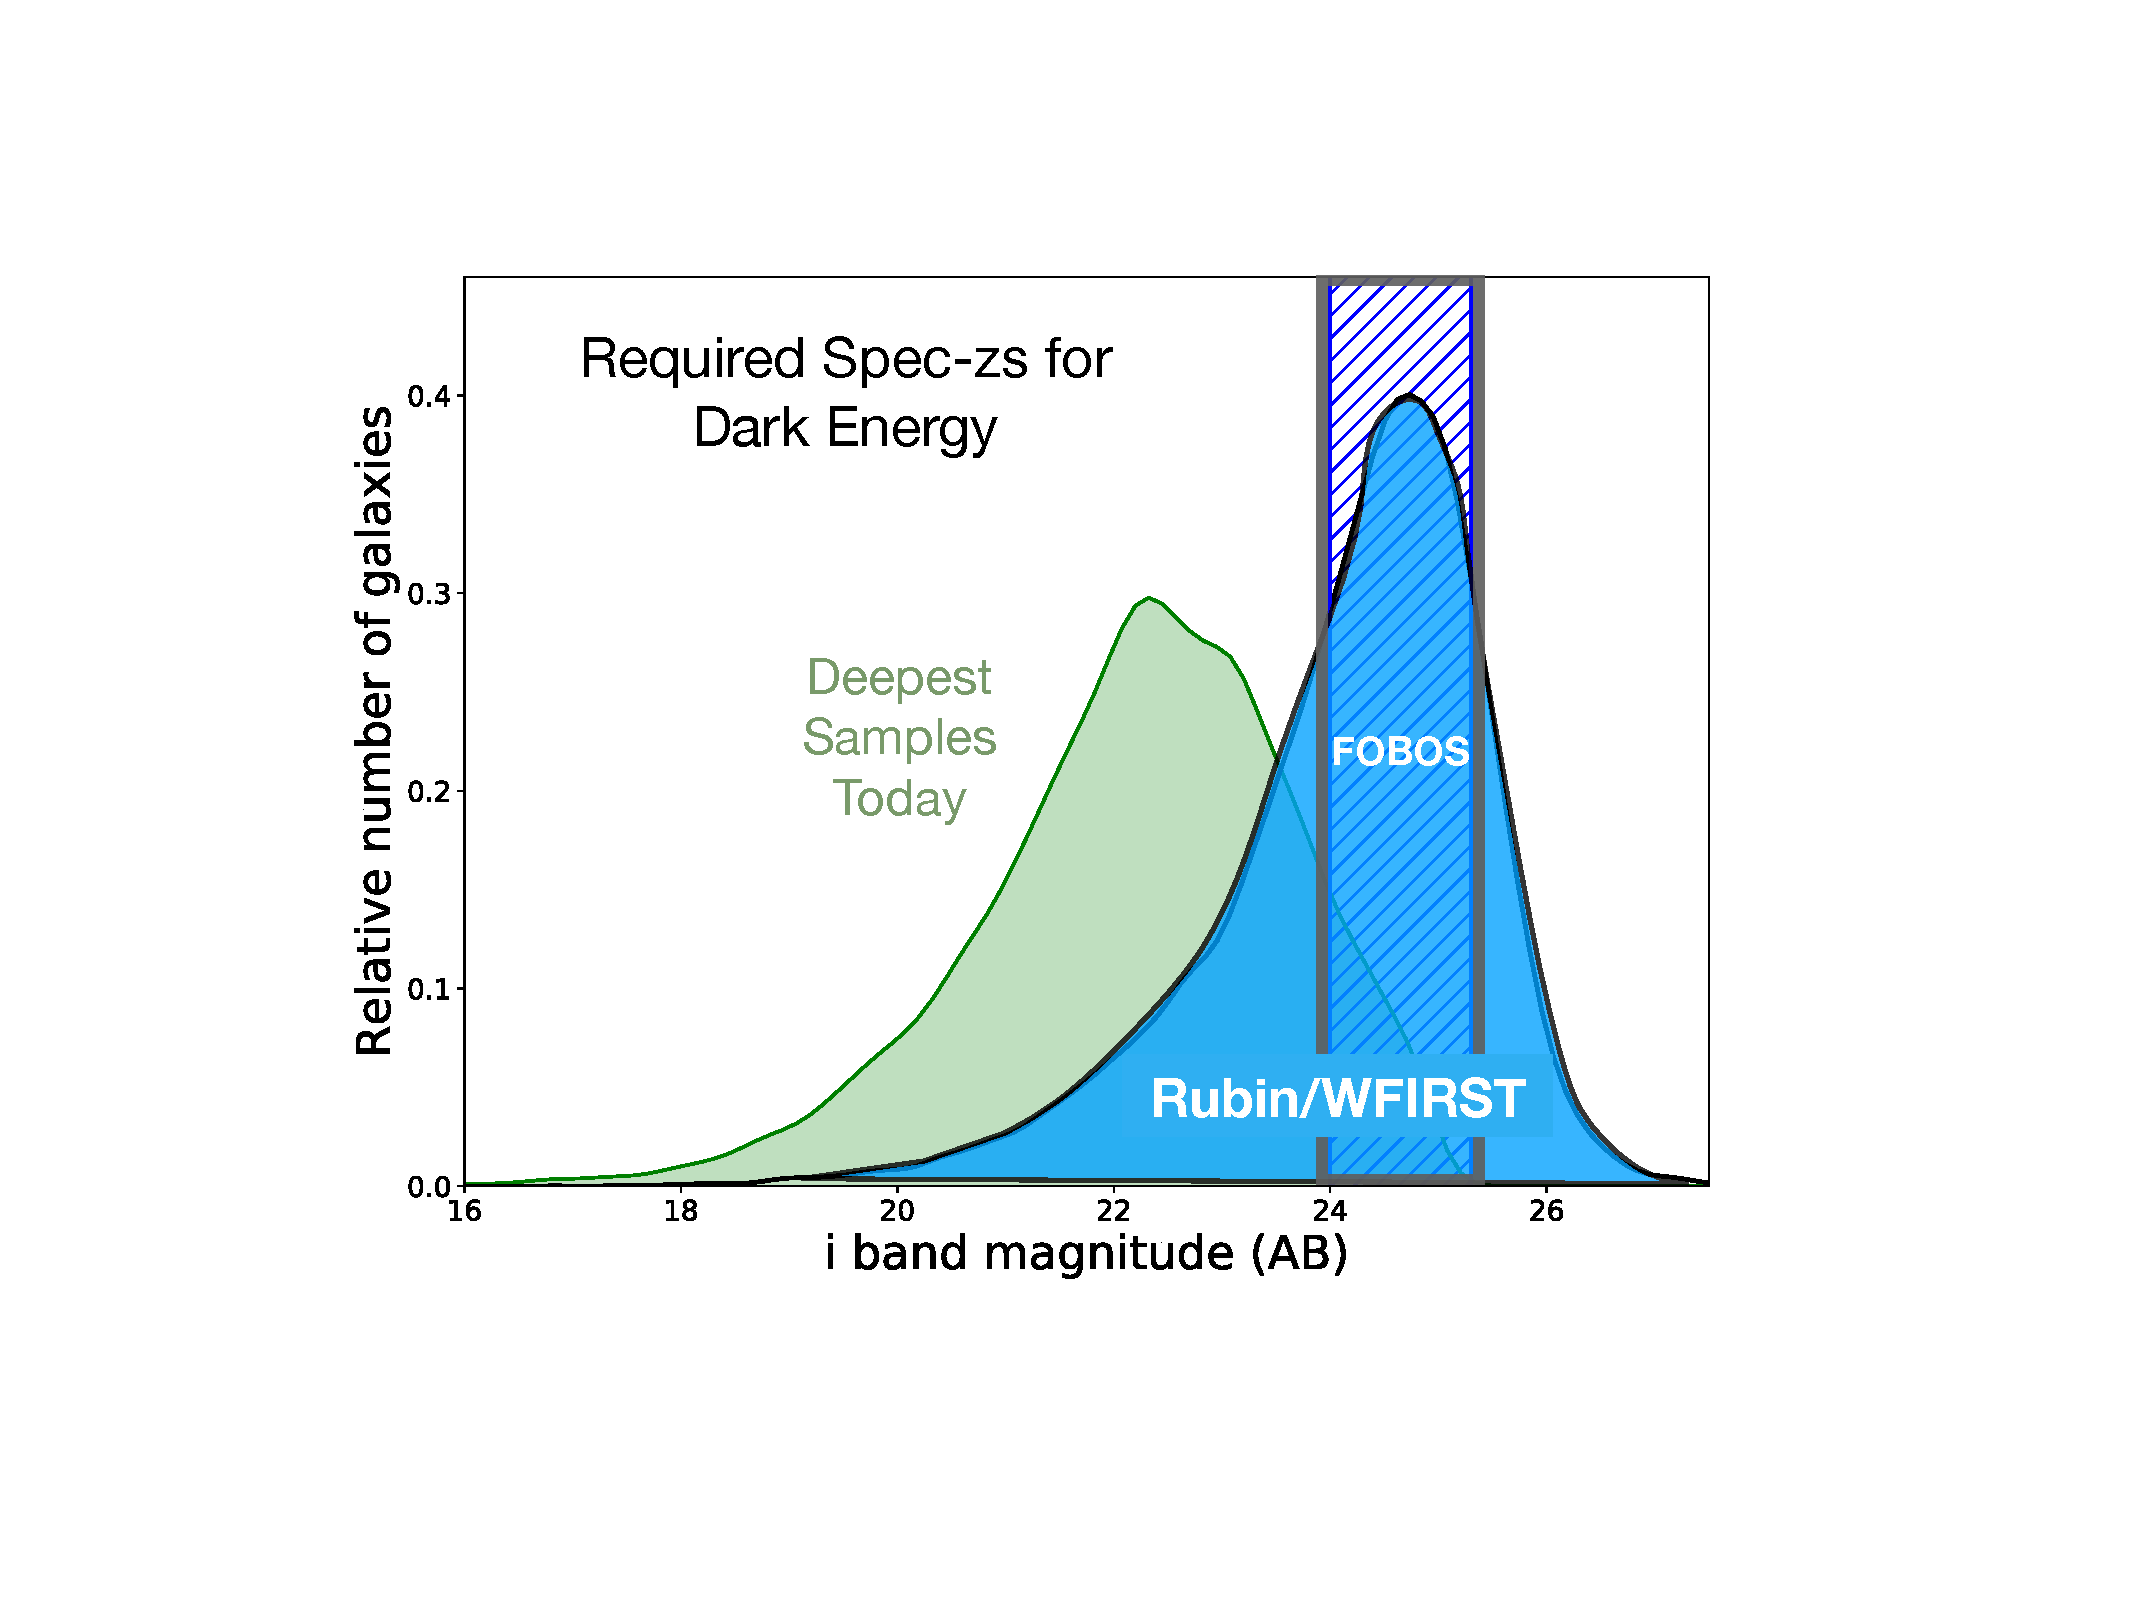
\includegraphics[width=0.7\textwidth]{figs/fobos_cosmology_v2.pdf}
\end{center}
\caption{\footnotesize Magnitude distribution of secure spec-$z$ samples in existing deep fields from, e.g., DEEP2, VVDS, VIPERS, C3R2, and zCOSMOS (\textit{green}), compared with the anticipated distribution of the LSST/WFIRST weak-lensing sample derived in \citet[][\textit{blue}]{hemmati18}. Ultra-deep (50hr) exposures in the FOBOS cosmology program are designed to obtain spec-$z$s for $\sim$15k faint galaxies in the hatched region, representing roughly 50\% of the weak-lensing sample of these missions and weakly constrained by current spec-$z$ samples. The FOBOS cosmology program would operate over 12 independent regions to mitigate cosmic variance, employing a careful selection to explore the full color-magnitude parameter space efficiently, as in \cite{masters15}. }
\label{fig:cosmos_magdist}
%\end{wrapfigure}
\end{figure}

FOBOS should position itself to uniquely meet the needs for photo-$z$ training, well into the advent of the 30-m class telescopes (E-ELT, TMT, GMT) in the 2030s.  FOBOS can provide photo-$z$ training data for sources with spectral features too blue or fluxes too faint for other instruments, like PFS,\footnote{Subaru's Prime Focus Spectrograph (PFS) commissioning in 2022.} but that dominate by number (Fig.~\ref{fig:cosmos_magdist}).  For example, Rubin Observatory will begin reaching the LSST target 5$\sigma$ point-source depth of $i_{\rm AB} = 26.8$ in 2029.   FOBOS spectroscopic follow-up to $i_{AB} = 25.3$ for extended sources will provide a well-matched training sample\footnote{\citet{newman15} emphasize that photo-$z$ ``calibration'' can be accomplished by cross-referencing all-sky surveys of various low-density tracers like quasars and associated absorbers, luminous red galaxies, and emission-line galaxies.} that will \textit{increase LSST's dark energy figure-of-merit by 40\%} \citep{newman15}. No other existing or planned instrument will obtain such a spectroscopic sample on this timescale.  Indeed, although \euclid\ and WFIRST will both perform grism spectroscopy, the relatively low-sensitivity and strongly biased samples (e.g., they will be far more sensitive to galaxies with strong emission lines) mean that grism spectra from these missions are insufficient to train photo-$z$s for the full weak-lensing samples.  Additionally, because FOBOS has no ``redshift desert'' (its blue wavelength coverage allows redshift determination at $1.5\lesssim z \lesssim2.5$ via Ly$\alpha$ or nearby UV absorption features), FOBOS observations will reduce the need for expensive, space-based\footnote{Ground-based near-IR spectroscopy is too contaminated by night-sky emission lines to provide spec-$z$s at the required level of completeness \citep{newman15}.} near-IR spectroscopy of galaxies with $z > 1.5$.  Beyond enhancing cosmological analyses, the resulting galaxy sample would have a major impact on galaxy-evolution studies by providing the spectroscopic coverage needed to fully leverage photometry for billions of galaxies. % (see \S\ref{sec:ML}). 

The following are a list of program requirements that enable FOBOS to meet the needs of photo-$z$ training in the LSST era.  \edit{check and justify all of these} test

\begin{programrequirement}
\reqitem The photo-$z$ training sample must include 15,000 galaxies in the magnitude range $24 < i_{\rm AB} < 25.3$ to populate the regions of the color-redshift mapping space relevant to the LSST-\euclid-Roman photometric samples. \label{prog:photoz:sample}
\reqitem The objects in the sample must be distributed roughly equally among 12 independent fields to limit cosmic variance, with field centers that span a large range in right ascension. \label{prog:photoz:fields}
\reqitem Each field must be at least 20\arcmin\ in diameter and contain roughly 1700 viable targets.  This number assumes 15,000 galaxies observed (\ref{prog:photoz:sample}) over the number of independent fields (\ref{prog:photoz:fields}), and it accounts for the expected redshift completeness (\ref{prog:photoz:zcomplete}).
\reqitem Each field must also overlap with the LSST footprint and be within the visibility window of Keck II for no less than one consecutive hour.
\reqitem At least 3 of these fields must overlap the LSST deep-drilling fields to enable bootstrapping the photo-$z$ training analysis to these deeper samples.
\reqitem Objects observed must achieve an $i$-band-weighted signal-to-noise of 3 per angstrom to ensure 75\% redshift completeness. \label{prog:photoz:snperspec}
\reqitem No target should require more than 50 hours of observing time to maintain observing efficiency.  Given requirement \ref{prog:photoz:snperspec}, this means the continuum S/N per object after one hour of observing must be no less than 0.4 per angstrom. \label{prog:photoz:snperhr}
\reqitem To efficiently build the sample, the program must be able to reconfigure individual fibers in a field to new targets either as targets acquire sufficient S/N for redshift measurements or targets are found to not meet requirement \ref{prog:photoz:snperhr}.
\end{programrequirement}

\begin{sciencerequirement}
\reqitem At least 75\% of FOBOS spectra for galaxies at $z<2.5$ with a continuum S/N of 3 per angstrom must result in accurate spectroscopic redshifts. \label{prog:photoz:zcomplete}
\reqitem For spectra satisfying \ref{prog:photoz:zcomplete}, statistical errors in the spectroscopic redshifts of continuum-only sources must be no large than $\sigma_z \sim xx$.
\reqitem For spectra satisfying \ref{prog:photoz:zcomplete}, statistical errors in the spectroscopic redshifts of emission-line sources sources must be no large than $\sigma_z \sim xx$.
\end{sciencerequirement}

% This program is designed to observe a set of twelve 0.1 deg$^2$ FOBOS pointings arranged evenly in right ascension and chosen to overlap with the LSST, \euclid, and WFIRST footprints.  At least three pointings would include LSST deep drilling fields (COSMOS, XMM-LSS, and E-CDFS).  The program satisfies the sample size, field variance, and depth requirements in \citet{newman15} by obtaining ultra-deep 50-hour integrations of $\sim$15,000 sources at $24 < i_{AB} < 25.3$, a magnitude range that covers the majority of LSST/WFIRST weak-lensing samples.  While near-Poisson performance with such extreme integration times has been demonstrated with fiber spectrographs \citep[e.g.,][]{gu17,childress17}, our team's investigation of critical design factors that enable such performance (Bundy et al., in prep) has defined FOBOS instrument requirements, including a multi-tier calibration system (\S \ref{sec:calib}).  Accounting for expected sensitivity and stability, our exposure-time calculator estimates a continuum S/N$\sim3.5$ ($i$-band) for the faintest sources at these depths, a level known to be sufficient for $>75$\% redshift success (e.g., \citealp{Newman13}, \citealp{masters19}). 

% With 1200 single fibers (per pointing) from two of FOBOS's three spectrographs assigned to cosmology program targets, parallel observations with IFUs fed to its 3rd spectrograph can leverage the ultra-deep exposures needed for targets in the \textit{FOBOS Galaxy Ecosystem Program} (\S \ref{sec:galaxies}).  Photo-$z$ calibrators targeted by single fibers will efficiently span color-magnitude space \citep{masters15, masters19} with dynamic re-allocation of fibers to new targets as successful redshifts are obtained.  This program would request 12.5 dark nights per year.

% TODO: **Move this somewhere relevant**:
% The source density of 40 arcmin$^{-2}$ far exceeds FOBOS's
% fiber density (6 arcmin$^{-2}$).
  

%----------------------------------------------------------

\section{Tomographic mapping of the Intergalactic Medium}

The fueling and regulation of galaxy growth during the peak formation epoch ($z \sim2$--3) is critically tied to the turbulent and gas-rich ecosystem in which early galaxies evolve. The James Webb Space Telescope (JWST) and upcoming 30-m class telescopes (ELTs) will marshal powerful infrared observations to study the stars and nebular gas at the heart of these early galaxies. But mapping the large-scale gaseous environments and filamentary networks that fuel and ultimately regulate galaxy evolution at these redshifts requires high multiplex absorption-line tomography and rest-frame UV spectral coverage.

% FOBOS enables an ambitious two-prong approach to characterizing galaxy ecosystems on all scales: a detailed tomographic study of the cosmic web at $z>1.5$ combined with an ultra-deep IFU survey of emission from the circumgalactic medium (CGM) of $\sim$180 galaxies at the peak of cosmic star formation.

The PFS Strategic Survey Program on Subaru (running 2023--2028) \edit{ref?} will complete an important first step in Ly$\alpha$ tomography of the intergalactic medium (IGM) by making a map of structure at $2.1 < z < 2.5$ over 15 deg$^2$.  This map will be relatively coarse, however, with a sight-line density of 1600 deg$^{-2}$.  Although this provides valuable statistical measures of cosmic-web structures, a detailed study of the interplay between the fueling and feedback mechanisms mediated by these structures requires chemical and kinematic diagnostics that are only possible with more fine-grain resolution and higher S/N.

% TODO:
%   - Need some examples of how these data would be used.
%   - Describe overlap with cosmology program.

An observing program with FOBOS can meet these needs by building a high-resolution map of the IGM via a dense network of Ly-$\alpha$ absorbers associated with targeted structures at $1.5 < z < 2.5$ \citep[see][]{lee16}.  If the PFS survey is completed and distributed in time, this program should prioritize follow-up targets between $1.5 < z < 2.1$ (not accessible to PFS, but where sources are brighter) in these fields, such as protoclusters and galaxy overdensities.  This higher density yields statistical insight at 1 Mpc separations (the scale of individual massive halos) and the ability to stack sightlines to gain further in S/N so that various heavy-element ion transitions can be studied.  A FOBOS program to acquire these data would need to meet the following requirements:

\begin{programrequirement}
\reqitem For sufficient statistics, targets should be acquired in a set of 12 fields of $\sim$0.5 deg$^2$ each.
\reqitem For sufficient spatial resolution of the reconstructed IGM tomography (\ref{prog:igm:dens}), each field should include $\sim$5000 targets between $1.5 < z < 2.5$. 
\reqitem Each field should also contain $\sim$3000 galaxies embedded in the cosmic web for comparison of the intergalactic and interstellar media.
\end{programrequirement}
\begin{sciencerequirement}
\reqitem Achieve source density commensurate with scales of massive halos; i.e., $\sim$1 Mpc for the most massive galaxy clusters at $z\sim 2$. \label{prog:igm:dens}
\reqitem To detect a minimum \ion{H}{1} column density of X with a statistical error of no more than 0.x dex, FOBOS spectroscopy must obtain an ${\rm S/N} \sim 3.5$ at $r_{\rm AB} \approx 24.6$. 
\end{sciencerequirement}

%{Baseline source density goals for PFS: 1600/deg$^2$ over 15 deg$^2$.  This sightline density translates to 100 sources over the FOBOS FOV.  From the luminosity function of LBGs, going to a depth of R = 24.5 affords 400 possible $z=2.0-3.0$ sources within a single FOBOS pointing.  A 3-hr observation delivers S/N$\sim4$ per pixel in the g band.  Going to R = 24.6 means 1000 possible sources per FOV at S/N$\sim3.5$.  If we improve on source density over PFS by a factor of 4, we reduce the average sightline separation to $\sim1$ per comoving Mpc, or resolving scales of most massive individual halos!  This leaves 1400 fibers for `embedded' galaxies in the foreground. }

% \note{Joe/Dan/Kyle: play-out the combination of the 2nd program above and the Cosmology program as a practical illustration of what a series of observing nights devoted to these programs might look like. }


\section{Chemistry and dynamics of the Circumgalactic Medium at $z\sim2$}


High- and intermediate-ionization transitions, such as \ion{O}{6} ($\lambda_{\rm rest} = 1032, 1037$ \AA) and \ion{C}{4} ($\lambda_{\rm rest} = 1548, 1550$ \AA), probe $10^{5-6}$ K and $10^4$ K gas, respectively.  This temperature range marks the peak in gas cooling and therefore constrains how gas rains onto galaxies to fuel star-formation, as well as tracks feedback processes that establish and regulate the circumgalactic medium (CGM).  Observations of this gas has largely hinged on detection via \textit{absorption} measurements against a background source \edit{refs}.  The ability of these observations to probe the chemodynamical state of the CGM is therefore limited by the number of viable targets through each halo, and stacking of sightlines through many halos is generally required to provide a statistical view of their properties.  If the CGM is instead observed in \textit{emission}, each galaxy halo can be studied individually.

Current Keck instrumentation, namely KCWI, enables the mapping of Ly$\alpha$ emission for individual galaxy halos at $z\sim2$, and metal-line emission has already been studied in some extreme objects. However, significant progress in the field requires deeper observations of a significant sample ($\sim$100 objects) of relatively ``normal'' galaxies (Fig.~\ref{fig:cgmsample}).  Such as sample allows us to explore correlation between host-galaxy and local CGM properties that will provide key observational constraints of comological hydrodynamical simulations.

The requirements of an observational program that meets these needs are:

\begin{programrequirement}
\reqitem Observe at least 100 individual galaxy halos over a range of host mass and SFR, ranging from Milky-Way-like progenitor galaxies to the most massive brightest-cluster-galaxies today: $9.7 <$ log ($M_*/M_\odot$) $< 11.5$ \edit{need ref for upper mass limit; Patel+2013a; add SFR limits}. \label{prog:cgm:sample}
\reqitem Must be able to obtain ultra-deep observations of each target by observing for up to 100 hr on an individual target.
\reqitem The target density of viable targets is expected to be \edit{XX} per arcmin$^2$.  Given the exposure-time requirements, multiplexing must be at least 10 objects observed per field to efficiently build the required sample (\ref{prog:cgm:sample}).
\end{programrequirement}

% ; i.e. $\lambda_{\rm obs} \lesssim 3100$ \AA

\begin{sciencerequirement}
\reqitem Measure line emission from gas diagnostic transitions to detect and distinguish cool $10^4$ K and warm-hot $10^{5-6}$ K gas phases in the CGM. \edit{Give specific lines and wavelengths.}
\reqitem Observations must produce contiguous maps of the regions beyond galaxy disk and disk/halo interface, requiring a field-of-view of $\gtrsim$10 kpc (co-moving).
\reqitem Spatial sampling must be sufficient to enable stacking of weak emission in the outer CGM.
% if necessary to construct emission profiles revealing thermodynamic structure of gaseous halo.  
\reqitem Must have a spectral range that observes \ion{O}{6} at $z\gtrsim2$.
\reqitem Resolve high-velocity outflows from ``ambient'' CGM gas at galaxy systemic velocity, $\sigma_v \sim 100$ \kms.  
\reqitem Spectral resolution must be able to measure line centroids to better than 10 \kms\ and Doppler broadening of line widths to better than $\sigma \sim 100$ \kms. 
\end{sciencerequirement}


% The combination of single-fiber and multiplexed IFU observations therefore allows FOBOS to map the density and dynamical state of diffuse gas at all relevant scales from the IGM to the CGM, providing novel constraints on the next generation of cosmological simulations.

% FOBOS's unique UV sensitivity and IFU capabilities also open completely new territory: FOBOS will deliver the first significant samples of high-$z$ galaxies with circumgalactic gas mapped \textit{in emission}. UV sensitivity opens access to 

%\begin{wrapfigure}{r}{0.6\textwidth}\small
%\vspace{-0.2cm}
\begin{figure}
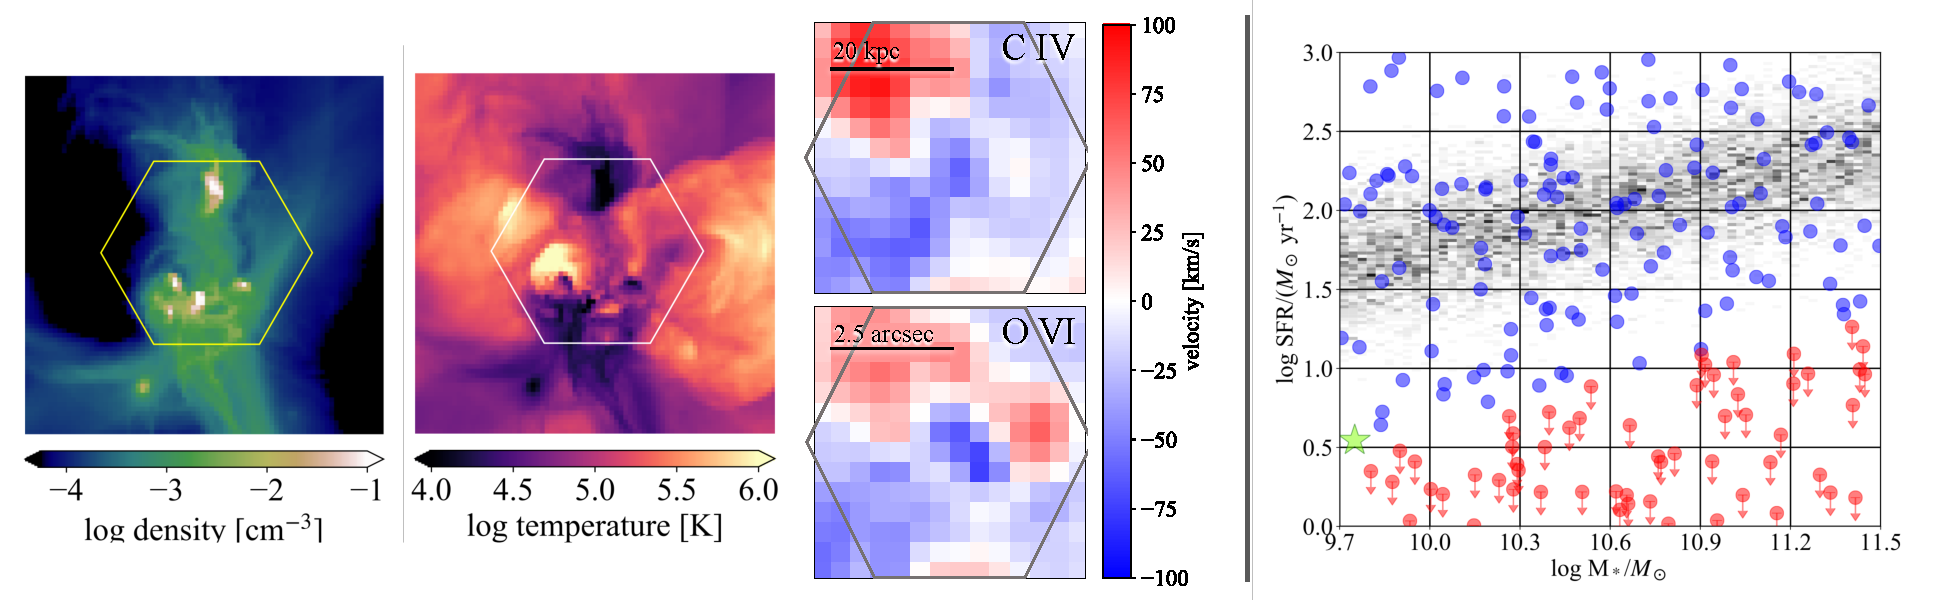
\includegraphics[width=\textwidth]{figs/msipProposalCgmCombo.pdf} %figs/CGMscience_v3.pdf}
\caption{\footnotesize \textit{Left}: Simulations of the density and temperature of the CGM at $z=2-2.5$ based on \citet{Corlies:2018aa}. \textit{Center}: Predicted observations of CGM emission sampled by the FOBOS IFUs, providing kinematic maps that trace gas flows using UV tracers (C IV and O VI).  \textit{Right}: The \textit{FOBOS Galaxy Ecosystem Program} will map these features for hundreds of galaxies sampling a large range physical parameters.  This panel shows a mock sample of program galaxies (star-forming in blue; passive in red) in the stellar mass-star formation rate ($M_*$-SFR) parameter space; the example simulation shown to the left is marked by a green star. The $M_*$-SFR ``main sequence'' from \citet{Whitaker:2012} is shown as the underlying gray 2D histogram.}
\label{fig:cgmsample}
\end{figure}
%\end{wrapfigure}

% In longer term, think through science that we should be proposing now-ish to do with JWST with the idea that we can follow-up with FOBOS.

% Billion galaxy survey?
%Field selection will take advantage of quasar-quasar pairs 
%at \note{range or exact number?} certain redshifts.

% In a joint observing scheme with the ultra-deep exposures of the \textit{FOBOS Cosmology Program}, the CGM study would use FOBOS's unique IFU multiplex capability (configuring one-third of FOBOS's fiber complement into into 15 37-fiber IFUs) to build an unprecedented sample of galaxies spanning respectively $\sim2$ and $>3$ orders of magnitude in $M_\ast$ and SFR, with maps of their CGM \textit{in emission}.  Each IFU will observe an on-sky diameter of 5.6 arcsec, sampling gaseous halos in each galaxy at 5 kpc scales out to a radius of 20--25 kpc (Fig.~\ref{fig:cgmsample}).  These observations require the equivalent of 12.5 dark nights per year.



\section{Kilonovae astrophysics}

The joint detection of electromagnetic radiation and gravitational waves from GW170817 began a new era of multi-messenger astronomy.  This single binary neutron star merger and its associated kilonova has remade our understanding of multiple branches of astrophysics, from the physical nature of mergers and explosion mechanisms to the origin of the heaviest elements in the universe.  By the late 2020s, gravitational wave detectors like LIGO,\footnote{The Laser Interferometer Gravitational-Wave Observatory} Virgo, and KAGRA\footnote{The Kamioka Gravitational Wave Detector, formerly the Large Scale Cryogenic Gravitational Wave Telescope (LCGT)} will routinely detect $\sim$30 binary neutron star mergers with kilonovae (KNe) annually \citep{abbott2018prospects}, providing the samples needed to understand how the physical properties and nucleosynthetic yields of KNe vary with environment.  Rapid spectroscopic follow-up of these events are critical to these studies, particularly for studying quickly decaying phases such as the 
Lanthanide-free ``blue" component of the KN light curve that peaks within a day post-merger at $\lambda_\mathrm{peak}\sim0.35$ $\mu$m (Fig.~\ref{fig:kilonova}).

Rubin Observatory target-of-opportunity (ToO) observations will search for KNe within an hour after the gravitational wave alerts are issued \citep[assuming the strategy proposed by][]{margutti2018}. For a typical 50 deg$^2$ localization region, we expect $\sim$100 KN candidates with $m_i\lesssim22.5$, the expected KN brightness at a sensitivity distance of 200 Mpc \citep{cowperthwaite2017, goldstein2019}. Identifying and triggering spectroscopic investigations of the true KN will require rapid and blue-sensitive follow-up capabilities. Such rapid follow-up of KN candidates discovered by LSST will enable a systematic population study of KNe and their environments.

%, each with a typical localization region of $\Omega_\mathrm{90\%}<100$ deg$^2$ . 

%\begin{wrapfigure}{r}{0.6\textwidth}%\small
\begin{figure}
\begin{center}
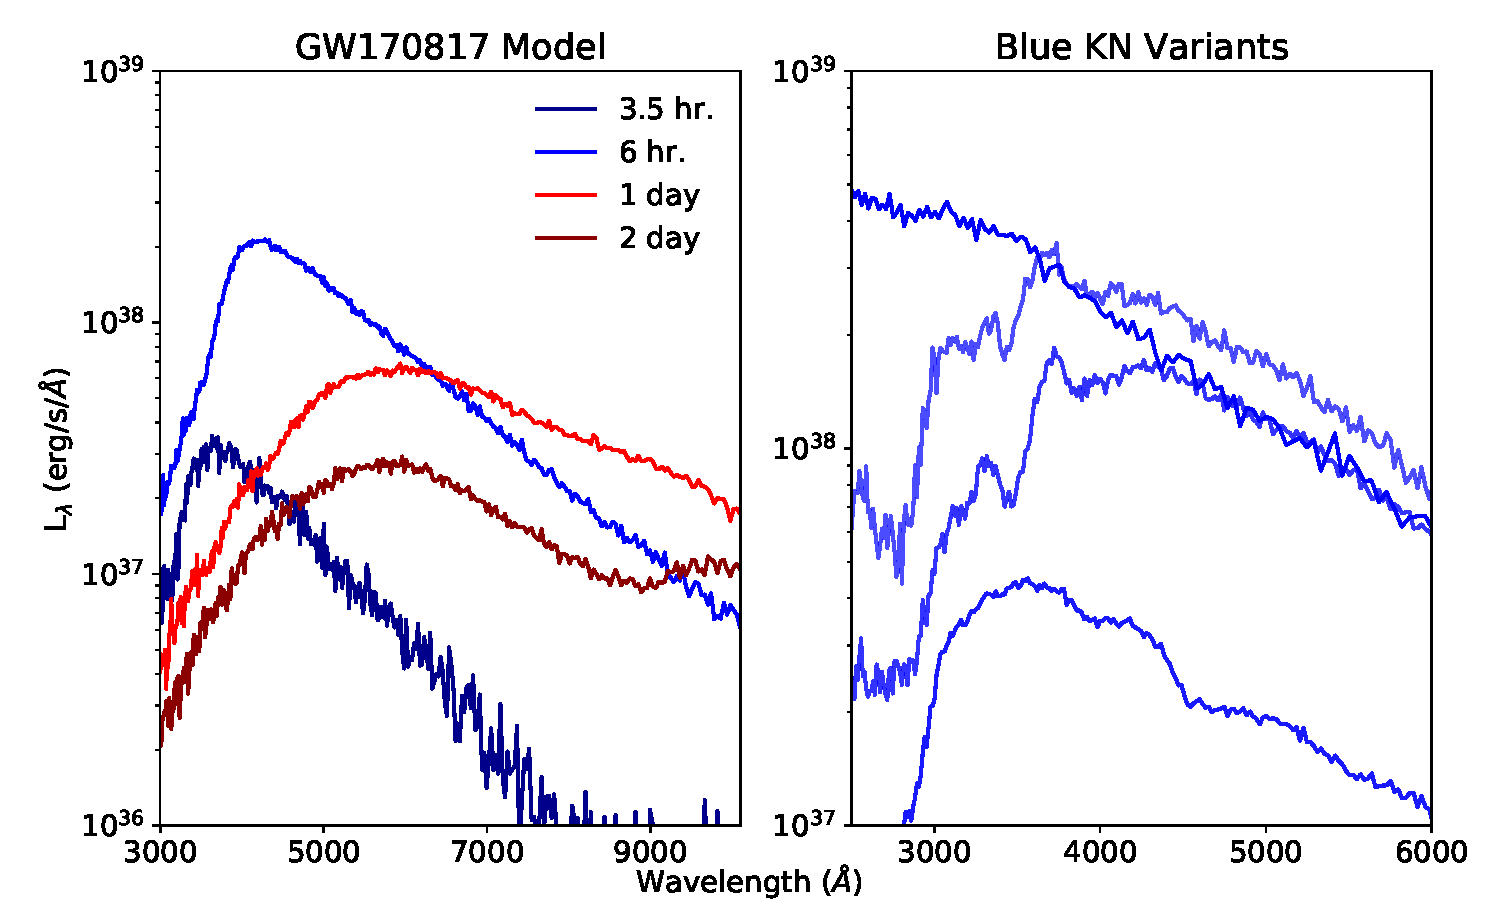
\includegraphics[width=0.8\textwidth]{figs/kn_fobos.pdf}
\end{center}
\caption{\textit{Left:} Model kilonova spectra based on GW170817 taken 3.5 hours, 6 hours, 1 day and 2 days post-merger. \textit{Right:} Variations of ``blue" kilonovae, generated by varying the energy, mass and Lanthanide fraction of kilonova models. FOBOS's blue sensitivity is essential to discriminate between these early-time models. Models from \citet{kasen2017}.}
\label{fig:kilonova}    
%\end{wrapfigure}
\end{figure}

Building spectroscopy of many KNe can be an expensive endeavor, both because LSST only provides KNe \textit{candidates} that must be spectrscopically vetted and because of their low on-sky density.  It is worth noting, therefore, that a highly multiplexed instrument is beneficial in this case because the KNe spectroscopy can be obtained jointly with other programs; however, this capability is not strictly a requirement of this specific program.

A program to vet KNe candidates and ultimately build a sample of high-quality KNe spectra at multiple evolution phases are as follows:

\begin{programrequirement}
\reqitem Assuming the strategies proposed by \citet{margutti2018}, we expect $\sim4$ KNe to be detectable by LSST and Keck annually. For each triggered event, we must observe $\gtrsim50$ candidates with short ($\sim$10 min), low-resolution ($R\sim1000$) spectroscopy.  This is nearly twice the total spectroscopic follow-up effort currently possible \citep{hosseinzadeh2019}.
\reqitem Observations should acquire spectroscopy of both the KNe and the host galaxy, ideally simultaneously within an integral-field unit.
\reqitem For confirmed KNe, the program should immediately transition to deeper ($\sim$1 hr) observations to potentially capture ``blue'' KNe (Fig.~\ref{fig:kilonova}).
\end{programrequirement}

%We would observe each candidate with FOBOS's central, fixed IFU to obtain a redshift and potential-host properties.  If our monitoring of real-time quick-look reductions identifies the KN, our strategy would immediately initiate deeper ($\sim1$ hour) observations to potentially capture ``blue" kilonovae   With four KNe annually, this FOBOS program requires $2.5$ nights per year; beyond the KNe observations, many fibers would be allocated to pre-assigned transient sources.

\begin{sciencerequirement}
\reqitem Candidate vetting spectra must achieve a S/N$\sim$3 magnitude limit of $g_\mathrm{AB}=24$ to identify KNe at limiting distance of $D_\mathrm{L}\sim300$ Mpc. 
\reqitem Redshift uncertainties of the host galaxy must be $\lesssim10$\%.
\end{sciencerequirement}

\section{Characterization of extragalactic LSST transients and their host galaxies}

Beyond KNe, Rubin Observatory will discover well over 1 million extragalactic transients annually, including thousands of currently-rare sources such as tidal-disruption events \citep{bricman2020}, superluminous supernovae \citep{villar2018} and changing look quasars. In a 20\arcmin\ field-of-view (the maximum field-of-view available to the Keck II Nasmyth port), we expect there to be $\sim$5 LSST transient hosts.  And within the LSST Deep Drilling Fields, we expect $\sim$150 total transients to be visible each year with $m_i<24$.  For a highly multiplexed instrument with dynamic target allocation, a high-impact, low-cost strategy would be to follow-up \textit{every} LSST transient and transient host within any given Keck pointing.  By combining both single-aperture and IFU observations of transients, we would dramatically increase the database of transient spectroscopy.  In particular, IFU observations of this regularity would dramatically increase the resolved spectroscopy of extragalactic hosts \citep[see a recent review by][]{anderson2015} at little additional cost. 
A series of requirements follow for observations of these targets:

\begin{programrequirement}
\reqitem Approximately 5-10 single-spectrum apertures should be held in reserve for serendipitous follow-up of LSST transient objects and their hosts for \textit{every} observing field acquired by Keck.
\reqitem A single IFU with a minimum field-of-view of 5\arcsec\ should be available to allow for modest localization errors.
\reqitem Target assignment must be responsive to on-the-fly triggering of newly discovered transients.
\end{programrequirement}

\begin{sciencerequirement}
\reqitem Sensitivity to $\lambda \lesssim 0.3$~$\mu$m is 
especially valuable for shock-driven (e.g., Type IIn supernovae) and relativistic events \citep[e.g., the atypically bright Type Ib supernova AT 2018cow;][]{margutti2019}.
\end{sciencerequirement}

% By deploying the remaining single fibers and IFUs on separate, pre-assigned transient sources in each pointing, we will take maximum advantage of synergies with time-series data from the world-wide follow-up observations of these gravitational-wave fields. 

% When deployed as the Keck II instrument, FOBOS's always-ready IFU makes it ideal for instant target acquisition and host galaxy characterization, all while simultaneously observing serendipitous targets of interest in the same field-of-view. 

\section{Chemodynamical structures in the stellar disks of M31 and M33}

start here

\begin{figure}
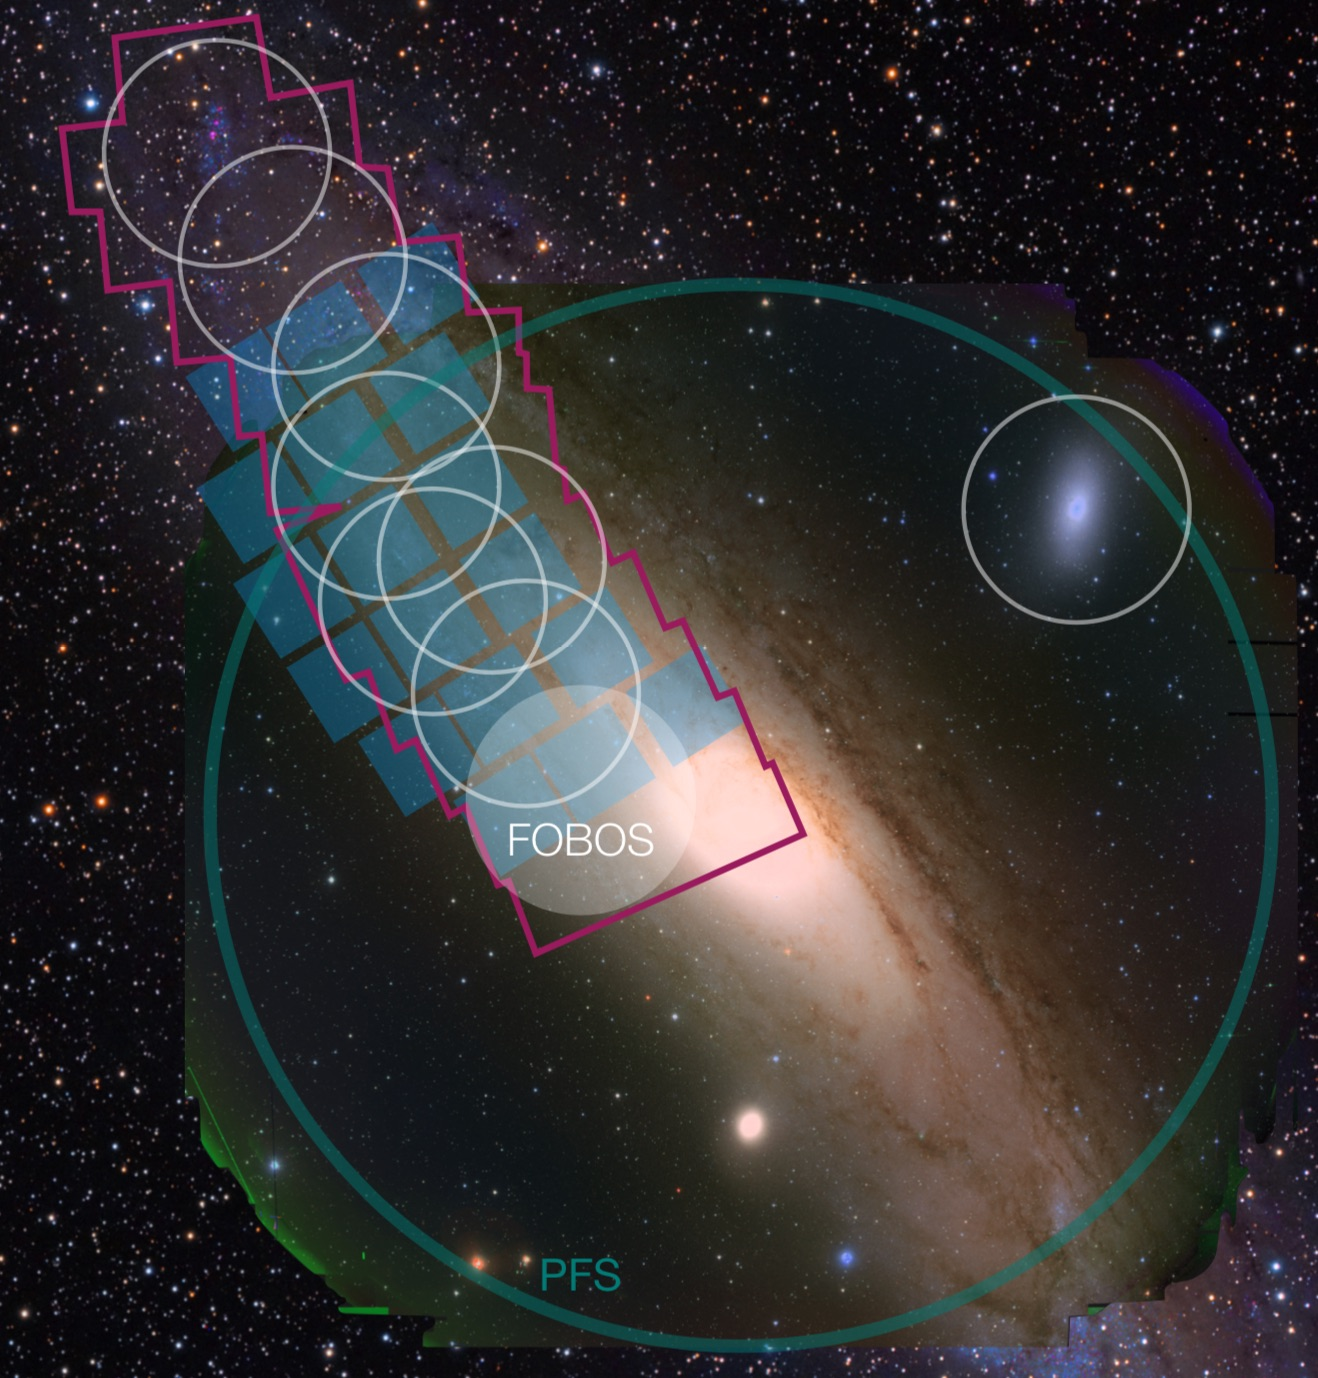
\includegraphics[width=0.58\textwidth]{figs/M31_footprint_v3.jpg}
\caption{A Subaru HSC image (lower right) superposed on a larger background image of M31 (credit: Adam Evans).  FOBOS pointings (white circles) span the PHAT area (magenta) and NGC 205.  The Subaru-PFS FOV (green circle; similar to MSE) and single-pointing WFIRST imaging footprint (blue squares) are also shown.}
\label{fig:M31}    
\end{figure}

\subsection{Assembly and Evolution of Andromeda's Disk and Satellite Galaxies}
\label{sec:localgroup}

Galaxy groups like the Local Group, with two L$^*$ galaxies, dominate the nearby universe \citep{kourkchi17}.  We expect galaxies in such groups to share common assembly histories, and yet, the Milky Way and Andromeda galaxies appear to have evolved in significantly divergent ways.  Differences from their star-cluster populations to their dwarf-galaxy properties remain poorly understood, limiting progress towards building a complete picture for how the Local Group formed and evolved.

For the Milky Way, stellar properties (e.g., age, metallicity, $\alpha$ abundance) and kinematics from large-scale spectroscopic surveys (e.g., APOGEE, GALAH, LAMOST) are now being combined with exquisite astrometric data from \textit{Gaia} to provide a revolutionary view of its evolution.  For example, these data reveal a clear bimodality in $\alpha$ abundance, indicating that stars at relatively greater distances from the disk plane (i.e., ``thick-disk'' stars) were formed in environments with much shorter star-formation timescales, likely due to a merger event that truncated star formation for a time.  Isolating chemically similar groups of stars in this way to reveal their common structural and dynamical properties is now fundamental to our understanding of the Milky Way.  This ``chemical tagging'' offers greater insights than studies of stars selected by their structural or dynamical associations alone.  With FOBOS, we can apply similar methods to the study of M31 and its satellite galaxies.

Although chemical tagging with M31 benefits from our outside view of this galaxy (compared to our inside view of the Milky Way), it also faces the challenge of obtaining precise stellar parameter measurements for very large samples.  First steps were made by SPLASH\footnote{Spectroscopic and Photometric Landscape of Andromeda’s Stellar Halo \citep[e.g.][]{splash}} which obtained $\sim$1hr Keck-DEIMOS exposures for $\sim$10,000 RGB stars in the disk, stellar streams, and halo of M31.  \citet{dorman15} used SPLASH to study the stellar age and velocity dispersion of disk stars and found that M31 features a much thicker, high-dispersion component than the Milky Way.  More recently, \citet{Escala20} explored metallicity and $\alpha$ abundance trends in 70 RGB stars ($\sim$6hr Keck-DEIMOS integrations) in the outer disk, inner halo, and Giant Stellar Stream of M31.  These trends also suggest a significant, merger-induced star-formation event in M31.  However, without more precise stellar parameters and larger samples --- beyond the limits of what one can expect to achieve with DEIMOS --- clear inferences that contrast the evolutionary histories of the Milky Way and M31 disks are out of reach.

\begin{figure}
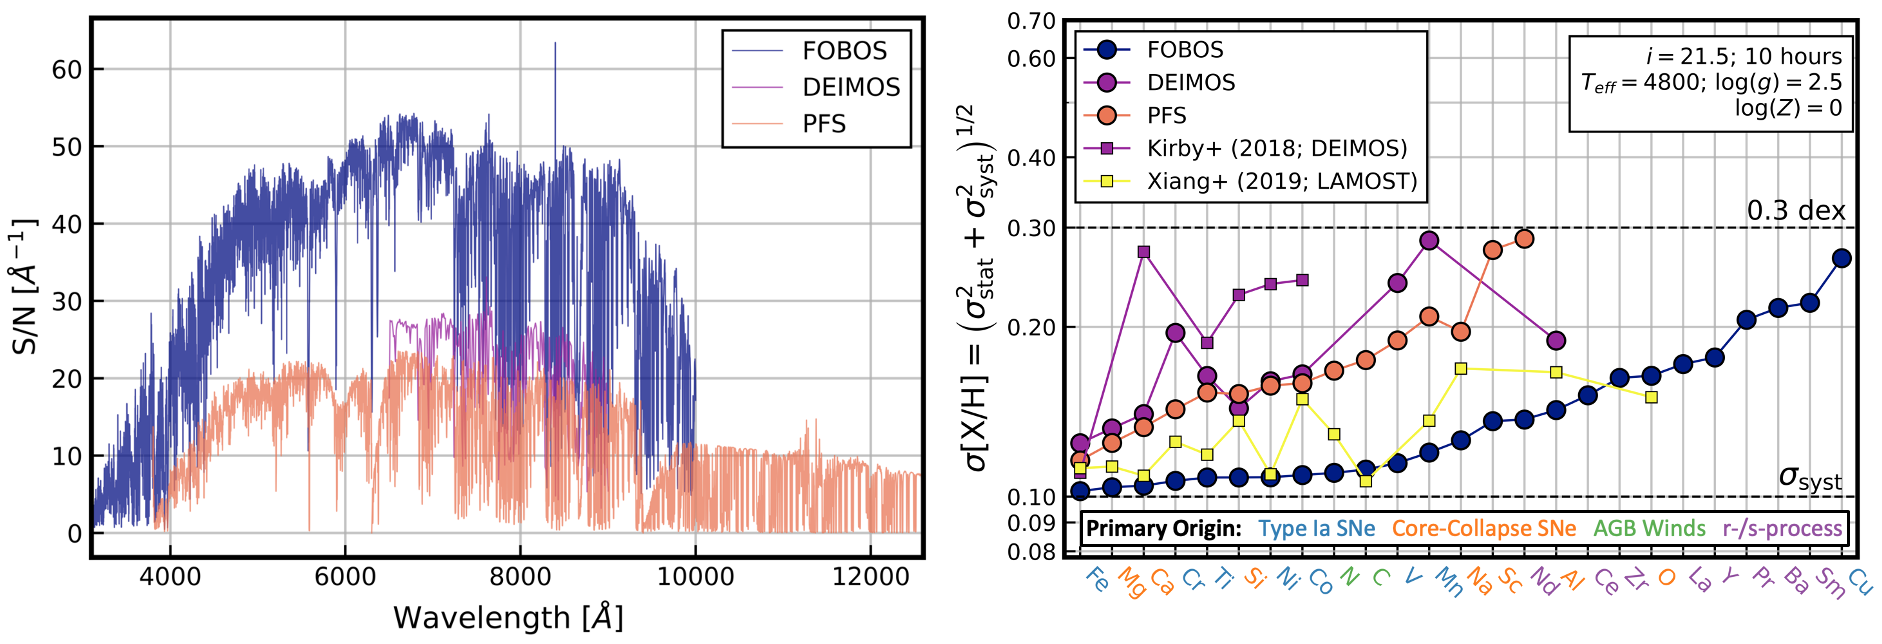
\includegraphics[width=1.0\textwidth]{figs/abundances_snr_v6.png}
\caption{Simulated observations demonstrating FOBOS's ability to perform ``chemical tagging'' in M31 and M33. \textit{Left:} Expected S/N for an $i=21.5$ RGB star in M31 observed for 10hr using FOBOS, PFS, and DEIMOS. \textit{Right:}  Forecasted abundance precision for these observations (filled circles), including both statistical uncertainty ($\sigma_{\rm stat}$; predicted by the Cram\'er-Rao Lower Bound) and a 0.1-dex systematic uncertainty \citep[$\sigma_{\rm syst}$; cf.,][]{kirby18, Xiang2019}. Elements are ordered along the ordinate by decreasing precision (limited to $\lesssim$0.3 dex) and color-coded by their primary nucleosynthetic origin. Although these forecasts are optimistic, the indicated \textit{relative} precision between instruments is robust. For reference, we show abundance uncertainties reported by \citet[][purple squares]{kirby18} from DEIMOS spectra of $-1.0<\text{[Fe/H]}<-0.6$ RGB stars in MW satellites with comparable S/N to our simulations; their measurement precision is worse than our DEIMOS predictions primarily because of their lower metallicity targets.  We also show abundance uncertainties reported by \citet[][yellow squares]{Xiang2019} from LAMOST spectra of MW RGB stars, scaled to the S/N and resolution of the proposed FOBOS  observations.}
\label{fig:abundances_snr}
\end{figure}

The \textit{FOBOS Andromeda Program} overcomes this challenge by building a sample that is both 10 times larger than SPLASH and $\gtrsim$0.5 mag deeper than \citet{Escala20}.\footnote{Compared to the \citet{Escala20} M31 disk sample alone, the \textit{FOBOS Andromeda Program} sample would be 5000 times larger.}  With FOBOS's larger wavelength coverage and improved S/N, we will measure precise velocities ($<$ 1 \kms), [Fe/H] and [$\alpha$/Fe] to $\sim$0.1 dex, individual elemental abundances to $\lesssim$0.2 dex \citep[Fig.~\ref{fig:abundances_snr}; cf.][]{YST2017}, and stellar age from blue CN absorption features.  Complementing the upcoming wide-field ($\sim$20 kpc at M31 distances) mapping of the M31 halo with PFS and MSE,\footnote{The Maunakea Spectroscopic Explorer (MSE) is a concept being developed for a future telescope and instrument at the current Canada-France-Hawaii Telescope site.} these data will provide the first clear, spatially-resolved measurements of chemodynamical trends in M31's disk, allowing us to address two key questions for the first time: Does M31, like the Milky Way, exhibit its own [$\alpha$/Fe] bimodality?  If so, were the ancient merger histories of the two galaxies linked or largely independent?

Finally, the \textit{FOBOS Andromeda Program} also includes legacy campaigns of 500 young stellar clusters in M31's disk \citep[dwarfing even Milky Way samples,][]{johnson15}, the dense cores of M31's major galaxy satellites, and 10,000 RGB stars in M33's disk.  In particular, observations of young stellar clusters capitalize on FOBOS's blue sensitivity and IFU capabilities to produce integrated-light spectra of these objects used to probe the recent evolution of the star-forming disk.  By comparing our measurements in the M31 and M33 disks, M31 young clusters, and M31 satellites with the halo population from PFS, we will construct a holistic picture of the evolution of M31 and its local environment.

% In addition to providing clues to the evolution of these objects specifically,

% All told, the FOBOS Andromeda Progam will allow for the first detailed comparisons of the internal structure, chemistry, and kinematics of M31 and its companions.  

%the blue sensitivity of FOBOS, along with its ability to obtain many small IFU regions within each pointing, will provide detailed spectroscopic maps of $\sim$500 young star clusters, , portegies10.  These clusters probe

% , including its dynamics and chemistry, as well as the conditions under which stars are formed and dispersed throughout the disk.  Although insights into the recent evolution of the M31's disk have already been possible through their photometric properties \citep[e.g.,][]{johnson16}, FOBOS will provide abundance, velocity, and mass information that is currently unavailable, allowing both confirmation of the inferences from photometry as well as large samples of spectroscopic masses and abundances to track the recent formation of stars and metals in clusters across the disk. 

% Turning to M33's disk and major Andromeda satellites, similar high-density FOBOS spectroscopy will

% Wide-field ($\sim$20 kpc at M31 distances) mapping of the M31 halo, using instruments like PFS and MSE,\footnote{The Maunakea Spectroscopic Explorer (MSE) is a concept being developed for a future telescope and instrument at the current Canada-France-Hawaii Telescope site.} will soon probe the chemodynamical history of its stellar substructures; however, FOBOS will provide unique capabilities particularly suited to the high-source-density M31 disk (see Fig.~\ref{fig:M31}).

% , M33, and the cores of Andromeda's major satellites.  Such data enable the chemodynamical studies needed to address key questions about the structure and assembly of these objects. 

% However, FOBOS's blue sensitivity, order-of-magnitude greater sampling density, and IFU modes offer  unique capabilities for obtaining a high-source-density census of M31's disk (see Fig.~\ref{fig:M31}), M33, and the cores of Andromeda's major satellites.  Such data enable the chemodynamical studies needed to address key questions about the structure and assembly of these objects. 


%These relations will determine whether M31's thicker disk is the result of dynamical ``heating'' of stars initially formed in a cold, thin disk versus the ``settling'' of a more turbulent primordial disk into the dynamically cold structures seen today.

%\note{paragraph on information garnered by observations of large satellites and young clusters in M31}

%Our large sample size, more than an order of magnitude larger than currently available, will allow for the finer subdivision of the stellar populations and the more-detailed quantification of the chemodynamical structures in M31 and M33, needed for a robust comparison to similar structures in our Milky Way.  

%Currently, {\it only} the Milky Way disk has been measured with this kind of precision, and it required very large surveys with substantial resources to complte, such as LAMOST  \citep{xiang2017, Xiang2019} and APOGEE \citep{hayden2015}.  With FOBOS, we can add {\it two} more disks to this detailed sample as just one example program of the science enabled.


%\note{Yuan-Sen: Maybe a sentence or two summarizing the importance of age-velocity-dispersion relation: e.g., nature vs. nurture; upside down ISM cooling vs. secular evolution}

%\note{Include brief statements in the paragraph above about the methods used to get age, metallicity, abundance?: C/N features for RGB age, combining PHAT+WFIRST photometry and FOBOS spectroscopy, abundances for individual elements}


%\note{Yuan-Sen: the C/N features of the optical spectra are a good age indicator for RGBs. So we could get age-velocity dispersion, on top of metallicity-velocity dispersion relation.}

%\note{Yuan-Sen: PHAT CMD + FOBOS spectra should give pretty good spectroscopic-photometric constraints on stars}

%\note{note gains in RGB numbers by probing deeper down the sequence?} 

% Proof in the pudding:
%\note{ref; https://arxiv.org/abs/1908.09727 ?}.

% \noindent{\textsf{FOBOS Andromeda Program:}}  

\subsubsection{FOBOS Andromeda Program} The program is designed in two parts. (1) We would construct benchmark spectroscopic samples of 100,000 and 10,000 RGB stars in the disks of M31 and M33, respectively.  Accounting for a 60\% rejection rate \citep{dorman12} due to crowding of ground-based RGB catalogs ($i_{\rm Vega} < 22.5$), we target six M31 pointings in the PHAT\footnote{Panchromatic Hubble Andromeda Treasury \citep{phat} is a multi-cycle HST program that maps $\sim1/3$ M31's star-forming disk in 6 filters.} region between 5--20 kpc.  Each pointing is visited 10 times, and two disk pointings beyond 20 kpc are each visited once.  In M33, we target 3 pointings, each visited twice.  Each visit will target a unique set of stars --- the stellar density is high enough to efficiently target new stars for each visit with $\sim$95\% completeness --- for a total integration time of 10 hours, an order-of-magnitude longer than the SPLASH survey.  We expect $i$-band ${\rm S/N} \approx 40$ \AA$^{-1}$ and $\approx 20$ \AA$^{-1}$ at the  ``sweet-spot'' of the RGB ($i_{Vega} = 21.5$) and a magnitude fainter, respectively.  This ensures a radial-velocity precision of $<$1 \kms \textit{for all targets} and precise metallicity and abundance measurements, as illustrated in Fig.~\ref{fig:abundances_snr}.
%an internal [Fe/H] precision between 0.05 and 0.1 dex, and an internal [$\alpha$/Fe] precision of 0.1 dex for all spectra with ${\rm S/N} \geq 20$ \AA$^{-1}$. For many stars, individual iron-peak and $\alpha$ elements, as well as C and N, will also be measurable to $\lesssim 0.2$ dex. 
This combination of sample size and precision allows us to directly compare radial trends in chemodynamical structures between M31, M33, and the MW. (2) Jointly with single-fiber observations of RGB stars, we would acquire IFU observations ($\sim$5.6\arcsec{} diameter) of $\sim$500 young star clusters in the M31 disk.  It would also dedicate 3 pointings (each visited once) for MOS observations of RGB stars in the area including NGC 147, NGC 185, and And II, and use a single pointing (visited twice) for NGC 205.  These observations target 9,000 RGB stars in the central regions of Andromeda's major satellites, yielding their dynamical masses, star-formation histories, and chemical composition.  The two components of the \textit{FOBOS Andromeda Program} would require a total of 19 nights per year over 5 years. 


\begin{programrequirement}

\reqitem Sample size: 100,000 RGB stars and 500 young star clusters in the M31 disk and 10,000 RGB stars in the M33 disk.

\reqitem M31 Targets: 6 disk pointings in the PHAT region between 5-20 kpc, each visited 10 times and 2 disk pointings beyond 20 kpc, each visited once. Every visit will target a unique set of stars with $\sim$95\% completeness.

\reqitem M33 Targets: 3 disk pointings, each visited twice. Every visit will target a unique set of stars with $\sim$95\% completeness.

\reqitem Instrument configuration: $>$70\% MOS fibers and $<$30\% IFU fiber bundles ($\sim$5.6" diameter) in the M31 disk and 100\% MOS fibers in the M33 Disk.

\reqitem Exposure time: 10 hours of integration per visit.

\reqitem Duration: 18 nights per year over 5 years for a total of 90 nights (84 for the M31 disk and 6 for the M33 disk).

\end{programrequirement}

\begin{sciencerequirement}

\reqitem Radial velocities to $\lesssim 1$ \kms.

\reqitem[] [Fe/H] and [$\alpha$/Fe] measured to $\lesssim 0.1$ dex.

\reqitem[] [X/Fe] measured to $\lesssim 0.2$ dex for individual iron-peak elements (e.g., \edit{which?}), $\alpha$-elements (e.g., \edit{which?}), and neutron-capture elements (e.g., \edit{which?}).

\reqitem Stellar ages from CN absorption features to $\lesssim$ \edit{??} Gyr.

\end{sciencerequirement}

\begin{requirement}

\reqitem Field of View of \edit{??}

\reqitem Multiplexing of \edit{??}

\reqitem Fiber density of \edit{??}

\reqitem Spectral resolution of $R>$ \edit{????}

\reqitem Spectral coverage from \edit{??-??} \AA.

\reqitem $\text{S/N}>$ \edit{??}

\end{requirement}


\section{Abundance patterns in the constituents of the M31 halo}

\begin{programrequirement}

\reqitem Sample size: 9,000 RGB stars in four M31 Satellites (NGC 147, NGC 185, And II, and NGC 205).

\reqitem Targets: 3 pointings in the region of NGC 147, NGC 185, and And II, each visited once. 1 pointing in NGC 205, visited twice. Every visit will target a unique set of stars with $\sim$95\% completeness.

\reqitem Instrument configuration: 100\% MOS fibers.

\reqitem Exposure time: 10 hours of integration per visit.

\reqitem Duration: 5 nights over 5 years.

\end{programrequirement}

\section{Program overlap and synergies}

\edit{This section highlights the overlap of the different programs and shows how they can be integrated.  Think Table 2 from the MSIP and the discussion around it.}

%%%%%%%%%%%%%%%%%%%%%%%%%%%%%%%%%%%%%%%%%%%%%%%%%%%%%%%%%%%%%%%%%%%%%%%%
% Science Drivers
%%%%%%%%%%%%%%%%%%%%%%%%%%%%%%%%%%%%%%%%%%%%%%%%%%%%%%%%%%%%%%%%%%%%%%%%

%-----------------------------------------------------------------------
% Cosmology
%-----------------------------------------------------------------------
\chapter{Science Drivers: Cosmology} \label{sci:cosmology}

\section{Photometric Redshift Training for Dark Energy Surveys}
\label{sci:photoz}

See DESC Google Doc of Desiridata: \url{https://docs.google.com/document/d/1SgST0eiQC2WmVFWyu6HUBpFN7EERZhC5t\_7OXrwRMJg/edit\#heading=h.olp0r1g70nxf}

Dark energy is one of the most fundamental, unsolved problems in both cosmology and particle physics.  It has inspired enormous world-wide efforts --- culminating in LSST, \euclid, and WFIRST --- that seek highly precise measures of cosmic structure to constrain the evolving dark-energy equation-of-state.

These measures utilize angular correlations of galaxy positions, their gravitational lensing shear, and the cross-correlation between the two. Unfortunately, photometric distances (via photometric redshifts, or ``photo-$z$s'') are significantly less precise than spectroscopic redshifts (spec-$z$s), introducing significant biases.  The spectroscopic validation of photo-$z$s we propose with FOBOS is therefore critical to the success of \textit{all} imaging surveys in this respect. It would not only \emph{increase the dark energy figure-of-merit in LSST by 40\%} \citep{newman15} but, importantly, provide vital confidence in cosmological results.  FOBOS is particularly powerful in this application because it has no ``redshift desert'' thanks to its unique ability to measure spectroscopic redshifts above $z > 1.5$ via rest-frame UV features.  This eliminates the need for expensive, space-based\footnote{Ground-based near-IR spectroscopy is too contaminated by sky-line emission to provide spec-$z$s at the required level of completeness \citep{newman15}.} near-IR spectroscopy. 

\emph{From DESC Collaboration}: resolve the [OII] 3727 angstrom doublet (R > 4000), on a large-aperture telescope (>6m if at all possible), with modestly large field of view (>20 arcmin diameter) preferred

\subsection{Science Requirements for Redshift Training Samples}

\begin{sciencerequirement}
\reqitem Redshift precision of 150 \kms{} or better. Stage IV cosmology experiments need to constrain the mean redshift of shear bins to $\lesssim0.2\%$. Redshift samples used for calibration must achieve at least this level of precision per source, which sets this requirement. 
%
\reqitem Redshift success rate of 75\% measured in a magnitude bin of width 0.5 mag up to the magnitude limit.  Explanation...
%
\reqitem Magnitude limit of $i_{\rm AB} = 25.3$.  This limit corresponds to the expected depth of LSST lensing samples (REF).
%
\reqitem Minimum sample size of 15,000, required for sufficient coverage of the photometric color space and for training statistics (REF).
%
\reqitem 10 independent fields of minimum 20\arcmin{} diameter in order to average over systematics in the galaxy population owing to sample variance.
%
\reqitem Redshift range of $z = $[0.1, 3.5], spanning the distribution of LSST and WFIRST cosmology samples (REF).
%
\end{sciencerequirement}

\section{Redshift Distributions of CMB Lensing Cross-Correlation Photometric Samples}

High-S/N CMB maps from next-generation CMB observatories (e.g., Simons Observatory and CMB-S4) will provide a cosmic ``reference background'' for measurements of gravitational lensing induced by matter along the line of sight.  After cross-correlating with Lyman Break Galaxy (LBG) samples, a relatively flat lensing ``kernel'' with power at $z = 2$--5 enables powerful constraints on the Inflation-sensitive matter power spectrum, Horizon-scale General Relativity, cosmic curvature and neutrino masses, and early Dark Energy \citep{ferraro19}.  \citet{wilson19} explore these constraints in detail and highlight the need for spectroscopic determination of accurate redshift distributions for the employed LBG samples. FOBOS would address this need in two ways.  First, several deep-drilling fields targeting $\sim$1000 LBGs BX, $u$, $g$, and $r$ drop-out candidates per pointing ($\sim$10,000 deg$^{-2}$) would establish the interloper rate and intrinsic redshift distribution of LBG samples to sufficient precision (this program would likely overlap with the photo-$z$ program described above).  Second, $\sim$200 LBGs per pointing (2000 deg$^{-2}$) could be included as a background program when FOBOS observes other sources across the sky, eventually building a 50-100 deg$^2$ data set of sparse high-$z$ spectroscopy for LBG dN/d$z$ calibration via clustering redshifts \citep[see][]{wilson19}. 

\subsection{Science Requirements for CMB Lensing Calibration}

\begin{sciencerequirement}
%
\reqitem Redshift precision of 150 \kms{} or better.  Explanation...
%
\reqitem Redshift success rate of 75\% measured in a magnitude bin of width 0.5 mag up to the magnitude limit.  Explanation...
%
\reqitem Photometric selections of various LBG samples...
%
\reqitem Minimum sample size of 
%
\reqitem 10 independent fields of minimum 20\arcmin{} diameter in order to average over systematics in the galaxy population owing to sample variance.
%
\reqitem Redshift range of $z = $[2, 5], spanning the peak power of the CMB lensing kernel.
%
\end{sciencerequirement}
%-----------------------------------------------------------------------

\newpage

%-----------------------------------------------------------------------
% Galaxy Evolution
%-----------------------------------------------------------------------
\chapter{Science Drivers: Galaxy Evolution} \label{sci:galaxies}

With both single-fiber and multiplexed IFU observations, FOBOS will produce rich and comprehensive data sets at faint source magnitudes.  Its blue sensitivity affords UV absorption studies down to $z \sim 1.5$, enabling detailed mapping of the baryonic environment at the peak formation epoch.  Samples at $z=1$--$2$ will not only characterize how this environment and its impact on galaxies evolves but will also provide large training sets that can be used to extract spectroscopic-like information from the billion-plus galaxy samples observed in all-sky surveys.  These data will be used in concert with large samples of spatially-resolved FOBOS observations (in IFU mode) to set the context for highly-detailed studies of targeted samples with James Webb Space Telescope and the U.S.~Extremely Large Telescopes.  Finally, FOBOS can tie evolutionary behavior seen at early times to the present day by observing faint sub-structure and dynamical tracers in nearby galaxies.

\section{1B Galaxy Samples from Spectroscopic Training}
\label{sci:1Bgalaxies}

Apply deep-learning algorithms to infer physical properties of galaxies at $z$$\sim$2 using using photometry. The range of observed spectral types is well-constrained by broad-band imaging, suggesting a far greater potential for imaging data to reveal physical properties with sufficient training than conventional modeling of spectral energy distributions (SEDs) would suggest.  Machine learning techniques will require training sets with well measured star-formation histories, stellar-population properties, dust content, inflow/outflow properties, and stellar masses --- and determine design parameters for future training sets that will enable such inferences for millions of imaged galaxies at $z$$\sim$2. 

\subsection{Science Requirements for the 1B Galaxy Sample}

\begin{sciencerequirement}

\reqitem Light-weighted stellar ages and metallicities with precision of 0.1 dex in appropriate bins of color space.

\reqitem Star formation rate uncertainties from strong emission lines of 0.1 dex in appropriate bins of color space.

\reqitem Redshift precision of at least 30 \kms{} to allow for accurate stacked spectra in specific color bins.

\end{sciencerequirement}


\section{The Galaxy Environment and Ecosystem}
\label{sci:ecosystem}

With publicly-accessible surveys like MOSDEF \citep{kriek15}, the Keck MOSFIRE instrument has provided powerful new insights into early galaxies at the $z$$\sim$2 peak-formation epoch \citep[also see KBSS,][]{steidel14}. However, a complete picture of the galaxy ``ecosystem'' at this key epoch must also consider the gas-filled environments. Using Ly$\alpha$ absorption in background galaxies, a tomographic map of the intergalactic medium (IGM) in regions surveyed by MOSDEF and KBSS is a key first step. The promise of this approach, demonstrated at Keck by \citet{lee14}, motivates FOBOS's UV sensitivity, target flexibility, and multiplex for tomographic mapping of large-scale structure, including protoclusters \citep{lee16,kartaltepe19}, voids \citep{krolewski18}, and filaments \citep{horowitz19}. \citet{2018arXiv181005156S} take IGM tomography in a new direction, demonstrating with simulated observations that quasar ``light echoes'' --- spatial signatures of the expanding ionization front of a newly activated quasar --- can be detected and used to infer opening angles and deconstruct the quasar's accretion history (see Fig \ref{fig:LightEcho}). The required FOBOS spectra can simultaneously constrain the CIV mass density (via $\lambda\lambda$1548,1550 \AA) and patterns of CIV enrichment on both IGM and circumgalactic scales, revealing the imprint of galaxy fueling and feedback processes \citep[e.g.,][]{tumlinson17}.

At later times, as IGM material becomes more confined to galaxies and their dark matter halos, these halos increasingly merge to form larger structures.  FOBOS will be particularly important for mapping out environmental effects at $z=1$--$2$ on galaxy evolution at the group scale ($\mathcal{M_\ast/M_\odot} \lesssim 10^{13}$) and statistically linking galaxies to their host dark matter halos \citep{behroozi19}.  Tens of thousands of satellites down to sub-L$^*$ luminosities will be mapped and characterized. Thanks to deep, wide-field imaging surveys, like LSST, a 1M-object environmental survey at $z=1$--$2$ may then be possible using improved photo-$z$s, strong priors on spectral types, and new machine-learning techniques to deliver \textit{ spectroscopic} redshifts (with $\lesssim$300 \kms\ accuracy) at the lowest signal-to-noise possible (exposure times reduced by factors of 4--5).

\subsection{Science Requirements for the Galaxy Ecosystem}

\begin{sciencerequirement}

\reqitem Detection of key IGM/ISM lines like... probing what densities.

\reqitem Redshift precision of at least 300 \kms{} to enable satellite membership

\reqitem Errors on the measured outflow velocity of less than 20~km~s$^{-1}$.  Outflows speeds of $\sim100 -- 200$~km~s$^{-1}$ are expected in most star forming galaxies where interstellar Na~I can be detected in absorption (Chen et al.~2010). 

\reqitem ...

\end{sciencerequirement}


\section{Internal Structure of Galaxies}
\label{sci:internal}

MaNGA \citep{bundy15} and other large IFU surveys are defining the $z=0$ benchmark for how internal structure is organized across the galaxy population. To understand and test ideas for how this internal structure emerged, we require spatially-resolved observations at $z = 1$--2, just after the peak formation epoch. Indeed, Keck has helped pioneer such observations \citep[e.g.,][]{erb04, miller11,law09}. With only one galaxy observed at a time, samples have so far been limited to a few hundred sources; however, FOBOS will obtain resolved spectroscopy for thousands of galaxies using its IFU-mode with a 25 deployed IFUs. Bright optical emission-line tracers for this unprecedented sample of galaxies will reveal their gas-phase and kinematic structure. Stacking restframe $\lambda \approx 4500$ spectra will enable radial stellar population analyses to constrain how stellar components formed and assembled. Although initially limited to coarse spatial scales, ground-layer adaptive optics (GLAO) in combination with FOBOS would be transformative for this science. A corrected FWHM of 0.2-0.3 arcsec would enable fine-sampling IFUs to probe smaller galaxies and study sub-structure on 1--2 kpc scales.

Environmental effects and evolutionary processes evident at higher redshift have consequences that can be tested in present-day galaxies.  Using globular cluster and planetary nebulae as tracers, FOBOS will dramatically advance dynamical studies of nearby galaxies with $\mathcal{M_\ast/M_\odot} \lesssim 10^{11}$, capturing the majority of the $\sim$1000 GCs located within $\sim$50 kpc of typical hosts \citep[see][]{2013ApJ...772...82H} and tightly constraining their dark matter halos. FOBOS's multi-IFU mode will additionally provide powerful insight on the origin of dwarf galaxies, both compact and ultra-diffuse (UDGs), in the field and in nearby clusters like Coma and Virgo.

Measurements of [O~II], [O~III], \Halpha, \Hbeta\, [N~II] and [S~II] will determine nebular gas metallicities, ionization parameter, and gas densities with high confidence. Measurements of \Halpha\ and \Hbeta\ yield estimates of the star formation rate over timescales of $\sim$$10^7$ years and dust extinction in \HII\ regions.  The combination of [O~III], \Hbeta, [N~II] and \Halpha\ allows us to place galaxies on the BPT diagram. [O~I] and [S~II] along with the BPT lines as a function of position within the galaxy differentiate between shocks in the interstellar medium, ionization by post-AGB stars, or the presence of a ``low-ionization'' active galactic nucleus.

One complication in placing requirements on nebular emission lines is that we expect a wide variation in line equivalent widths (EWs) in our sample. Obviously, we cannot guarantee determining, for example, 0.2 dex in SFR when the emission lines are too weak. Therefore, we set the requirements for a minimum peak amplitude of \Hbeta\ being 70\% of the continuum. This is equivalent to \Hbeta\ EW of 2.5\AA\ for an intrinsic line sigma of 50 \kms\ or EW of 5\AA\ for an intrinsic line sigma of 160 \kms. We chose \Hbeta\ because it is often the weakest emission line of all and is the limiting factor in determining extinction and SFR.

The stellar populations in a galaxy represent a record of the galaxy's star formation and chemical enrichment history.   For quiescent galaxies ages, metallicities, and abundances ratios are typically been measured using line indices \citep[e.g.][]{johansson12}.  More recently, methods have been developed that make use of the full spectrum \citep{conroy14}.  For late-type galaxies, constraints the mean stellar age and the presence of recent bursts come from the 4000~\AA\ break and the high order Balmer lines \citep[e.g.][]{kauffmann03a}. 

FOBOS's wide spectral range (3500--10,000~\AA) captures a large range of absorption features, from blue indices such as D4000, Ca H$+$K, and higher-order Balmer lines, through classical optical absorption features such as \Hbeta, Mg\textit{ b}, and Fe5270/Fe5335, to red, gravity-sensitive features such as the Ca triplet at $8600$~\AA. These features encode a great deal of information about star formation histories and the IMF, and can be used to measure element abundance ratios like [Mg/Fe], [N/Fe], [C/Fe] and [Ca/Fe].

\subsection{Science Requirements: Galaxy Structure with IFUs}

\begin{sciencerequirement}

\reqitem Gas ionization diagnostics ([N II]/H$\alpha$ vs.\ [O III]/H$\beta$) to separate gas that is photoionized from gas that is shocked or ionized by an AGN. The required precision in the log of the line ratios is $\pm$0.2 dex to minimize classification uncertainty.

\reqitem Spatial resolution of better than XXX kpc for a large fraction of the central galaxies in the sample in order to spatially resolve?

\reqitem Per-fiber S/N limits for dwarf galaxies, both compact and ultra-diffuse (UDGs), in the field and in nearby clusters like Coma and Virgo.

\reqitem A spectral resolution $\rm R=\lambda/\Delta \lambda$ of at least 1,500 is needed to properly subtract the H$\beta$ stellar absorption from the corresponding nebular emission, to fully resolve the [NII] doublet from H$\alpha$, and to resolve the [SII] doublet.

\reqitem Stellar continuum $S/N > 7$ per pixel near \Hbeta\ per spatial resolution element so that we can constrain E(B-V) to 0.2 and achieve a ${\rm \Sigma_{SFR}}$ estimate of 0.2 dex. In the current baseline sample design and observing strategy, we can achieve this in half of the Primary sample. We expect that in most star forming galaxies, the H$\beta$ strength will be stronger than 70\% of the continuum at 1.5\Reff.Therefore, more than half of the galaxies will have ${\rm \Sigma_{SFR}}$ constrained to better than 0.2 dex per spatial resolution element.

\reqitem An A/N of $>7$ on the key nebular lines [O~II], H$\beta$, and [O~III] is needed to measure the gas metallicity with an accuracy better than 0.05~dex per elliptical annulus at 1.5\Reff. This translates to a continuum $S/N > 10$ per pixel near \Hbeta. An A/N of $>10$ on [N~II] is needed to locate galaxy sub-regions on the diagnostic diagrams with an accuracy better than 0.1 dex. Such S/N on [N~II] will also allow the determination of the [N/O] abundance ratio with an accuracy better than 0.1 dex.  % Individual fibers!

%Note that this requirement
%  on H$\beta$ is weaker than the requirement of measuring the
%  dust extinction (E(B-V)) with an accuracy better than 0.2 per spatial resolution element. 

\reqitem Galaxies should be sampled by a minimum of 2.5 fibers per 1.5\Reff\ to enable measurements of metallicity gradients 

\reqitem Spectral stacking?

\reqitem For tracer studies, determine the dark matter fraction within 1.5\Reff\ and 2.5\Reff\ to 10\% (?)


\reqitem (\emph{From MaNGA, how close do we get to this with FOBOS?}) Resolve the bulk of the baryons by having at least 2 spatial resolution elements across the half-light radius.

\reqitem  Gas kinematics will use standard tracers such as the Balmer lines (\Hbeta, \Halpha), [OI], [OII], [OIII], [NII] and [SII], sometimes fitted simultaneously. 

\reqitem  Emission-line tracers will be continuum corrected to account for associated absorption lines, the kinematics of which will derived independently from absorption lines that are not heavily contaminated by emission.

\reqitem Gas velocity accuracy of 6-10 \kms\ and dispersion to ~30 \kms\ for lines with peak S/N $>$10.  Equivalently, $k_1$ (the kinemetric first moment) from emission-line tracers, will be determined to an accuracy of $<$ 5 \kms\ for amplitude-over-noise $A/N>5$ and $<$ 10 \kms\ for $A/N<5$. This applies only to galaxies with line-emission, that are rotation dominated, and have at least 5 spatial resolution elements across the major axis. 

\end{sciencerequirement}
%-----------------------------------------------------------------------

\newpage

%-----------------------------------------------------------------------
% Local Group
%-----------------------------------------------------------------------
\chapter{Science Drivers: Milky Way and Local Group} \label{sci:localgroup}

\section{Halo Assembly in the Milky Way and M31}

Galaxy groups like the Local Group, with two L$^*$ galaxies, dominate the nearby universe \citep{kourkchi17}.  We expect galaxies in such groups to share common assembly histories, and yet, the Milky Way and Andromeda galaxies appear to have evolved in significantly divergent ways.  Differences from their star-cluster populations to their dwarf-galaxy properties remain poorly understood, limiting progress towards building a complete picture for how the Local Group formed and evolved.

Of particular interest, for example, is the ability of future imaging surveys to increase the census of stellar streams and other substructure by a hundredfold.  The stars in these structures are faint, however, and easily confused with background galaxies in ground-based photometry.  With spectrocopic reference samples from FOBOS, the goal is to photometrically reconstruct the star-formation histories of disrupted satellites and compare them with dynamical models to constrain assembly histories and enclosed mass constraints \citep[e.g.,][]{2017ApJ...836..234S}.


Studies of individual stars in the Milky Way (MW), Magellanic Clouds, Andromeda (M31), Triangulum galaxy (M33), and numerous dwarf satellites provide an exquisitely detailed look at specific examples of galaxy assembly and evolution. While Gaia provides on-sky motions and photometry for 1.7 billion stars in the MW, fewer than 10\%, 0.3\%, and 0.1\% of stars will have a full complement of astrometrics and kinematics, basic stellar parameters, and chemical abundances, respectively.  Moreover, Gaia distance errors increase quadratically with distance.  Spectroscopy with APOGEE, the Milky Way Mapper, and WEAVE provide supporting wide-field data sets but accounting for fainter stars requires FOBOS-like sensitivity \citep[see][]{dey19,sanderson19}.  By carefully exploiting the overlap in these data sets, FOBOS can link high-resolution and robust stellar information from brighter targets to stars that can only be characterized by photometry.  This would enable data-driven models capable of providing photometric estimates of stellar parameters (temperature, surface gravity, metallicity, and alpha-element abundance) for \textit{ all} stars in the Gaia dataset  \citep[see][]{2015ApJ...808...16N, 2018arXiv180401530T, 2018arXiv180803278T}. 


For the Milky Way, stellar properties (e.g., age, metallicity, $\alpha$ abundance) and kinematics from large-scale spectroscopic surveys (e.g., APOGEE, GALAH, LAMOST) are now being combined with exquisite astrometric data from \textit{ Gaia} to provide a revolutionary view of its evolution.  For example, these data reveal a clear bimodality in $\alpha$ abundance, indicating that stars at relatively greater distances from the disk plane (i.e., ``thick-disk'' stars) were formed in environments with much shorter star-formation timescales, likely due to a merger event that truncated star formation for a time.  Isolating chemically similar groups of stars in this way to reveal their common structural and dynamical properties is now fundamental to our understanding of the Milky Way.  This ``chemical tagging'' offers greater insights than studies of stars selected by their structural or dynamical associations alone.  With FOBOS, we can apply similar methods to the study of M31 and its satellite galaxies.

Although chemical tagging with M31 benefits from our outside view of this galaxy (compared to our inside view of the Milky Way), it also faces the challenge of obtaining precise stellar parameter measurements for very large samples.  First steps were made by SPLASH\footnote{Spectroscopic and Photometric Landscape of Andromeda’s Stellar Halo \citep[e.g.][]{splash}} which obtained $\sim$1hr Keck-DEIMOS exposures for $\sim$10,000 RGB stars in the disk, stellar streams, and halo of M31.  \citet{dorman15} used SPLASH to study the stellar age and velocity dispersion of disk stars and found that M31 features a much thicker, high-dispersion component than the Milky Way.  More recently, \citet{Escala20} explored metallicity and $\alpha$ abundance trends in 70 RGB stars ($\sim$6hr Keck-DEIMOS integrations) in the outer disk, inner halo, and Giant Stellar Stream of M31.  These trends also suggest a significant, merger-induced star-formation event in M31.  However, without more precise stellar parameters and larger samples --- beyond the limits of what one can expect to achieve with DEIMOS --- clear inferences that contrast the evolutionary histories of the Milky Way and M31 disks are out of reach.

The \textit{ FOBOS Andromeda Program} overcomes this challenge by building a sample that is both 10 times larger than SPLASH and $\gtrsim$0.5 mag deeper than \citet{Escala20}.\footnote{Compared to the \citet{Escala20} M31 disk sample alone, the \textit{ FOBOS Andromeda Program} sample would be 5000 times larger.}  With FOBOS's larger wavelength coverage and improved S/N, we will measure precise velocities ($<$ 1 \kms), [Fe/H] and [$\alpha$/Fe] to $\sim$0.1 dex, individual elemental abundances to $\lesssim$0.2 dex \citep[Fig.~\ref{fig:abundances_snr}; cf.][]{YST2017}, and stellar age from blue CN absorption features.  Complementing the upcoming wide-field ($\sim$20 kpc at M31 distances) mapping of the M31 halo with PFS and MSE,\footnote{The Maunakea Spectroscopic Explorer (MSE) is a concept being developed for a future telescope and instrument at the current Canada-France-Hawaii Telescope site.} these data will provide the first clear, spatially-resolved measurements of chemodynamical trends in M31's disk, allowing us to address two key questions for the first time: Does M31, like the Milky Way, exhibit its own [$\alpha$/Fe] bimodality?  If so, were the ancient merger histories of the two galaxies linked or largely independent?

Finally, the \textit{ FOBOS Andromeda Program} also includes legacy campaigns of 500 young stellar clusters in M31's disk \citep[dwarfing even Milky Way samples,][]{johnson15}, the dense cores of M31's major galaxy satellites, and 10,000 RGB stars in M33's disk.  In particular, observations of young stellar clusters capitalize on FOBOS's blue sensitivity and IFU capabilities to produce integrated-light spectra of these objects used to probe the recent evolution of the star-forming disk.  By comparing our measurements in the M31 and M33 disks, M31 young clusters, and M31 satellites with the halo population from PFS, we will construct a holistic picture of the evolution of M31 and its local environment.

The program is designed in two parts. (1) We would construct benchmark spectroscopic samples of 100,000 and 10,000 RGB stars in the disks of M31 and M33, respectively.  Accounting for a 60\% rejection rate \citep{dorman12} due to crowding of ground-based RGB catalogs ($i_{\rm Vega} < 22.5$), we target six M31 pointings in the PHAT\footnote{Panchromatic Hubble Andromeda Treasury \citep{phat} is a multi-cycle HST program that maps $\sim1/3$ M31's star-forming disk in 6 filters.} region between 5--20 kpc.  Each pointing is visited 10 times, and two disk pointings beyond 20 kpc are each visited once.  In M33, we target 3 pointings, each visited twice.  Each visit will target a unique set of stars --- the stellar density is high enough to efficiently target new stars for each visit with $\sim$95\% completeness --- for a total integration time of 10 hours, an order-of-magnitude longer than the SPLASH survey.  We expect $i$-band ${\rm S/N} \approx 40$ \AA$^{-1}$ and $\approx 20$ \AA$^{-1}$ at the  ``sweet-spot'' of the RGB ($i_{Vega} = 21.5$) and a magnitude fainter, respectively.  This ensures a radial-velocity precision of $<$1 \kms\ \textit{ for all targets} and precise metallicity and abundance measurements, as illustrated in Fig.~\ref{fig:abundances_snr}.
%an internal [Fe/H] precision between 0.05 and 0.1 dex, and an internal [$\alpha$/Fe] precision of 0.1 dex for all spectra with ${\rm S/N} \geq 20$ \AA$^{-1}$. For many stars, individual iron-peak and $\alpha$ elements, as well as C and N, will also be measurable to $\lesssim 0.2$ dex. 
This combination of sample size and precision allows us to directly compare radial trends in chemodynamical structures between M31, M33, and the MW. (2) Jointly with single-fiber observations of RGB stars, we would acquire IFU observations ($\sim$5.6\arcsec{} diameter) of $\sim$500 young star clusters in the M31 disk.  It would also dedicate 3 pointings (each visited once) for MOS observations of RGB stars in the area including NGC 147, NGC 185, and And II, and use a single pointing (visited twice) for NGC 205.  These observations target 9,000 RGB stars in the central regions of Andromeda's major satellites, yielding their dynamical masses, star-formation histories, and chemical composition.  The two components of the \textit{ FOBOS Andromeda Program} would require a total of 19 nights per year over 5 years. 


%-----------------------------------------------------------------------

\newpage


\newpage

%-----------------------------------------------------------------------
% Time Domain
%-----------------------------------------------------------------------
\chapter{Science Drivers: Time Domain Astrophysics} \label{sci:timedomain}

\section{Rapid Spectroscopy of Kilonova Candidates}

\textit{copied from MSIP}
The joint detection of electromagnetic radiation and gravitational waves from GW170817 began a new era of multimessenger astronomy.  This single binary neutron star merger and its associated kilonova has remade our understanding of multiple branches of astrophysics, from the physical nature of mergers and explosion mechanisms to the origin of the heaviest elements in the universe.  Once FOBOS goes on-sky in the late 2020s, gravitational wave detectors like LIGO, Virgo and KAGRA will routinely detect $\sim$30 binary neutron star mergers with kilonovae (KNe) annually, providing the samples needed to understand how the physical properties and nucleosynthetic yields of KNe vary with environment.  FOBOS will be crucial in obtaining rapid spectroscopy of the Lanthanide-free ``blue" component of the KN light curve, which peaks within a day post-merger at $\lambda_\mathrm{peak}\sim0.35$ $\mu$m. When deployed as the Keck II instrument, FOBOS's always-ready IFU makes it ideal for instant target acquisition and host galaxy characterization, all while simultaneously observing serendipitous targets of interest in the same field-of-view. 


\subsection{Science Requirements: Kilonova Candidate Identification}

\begin{sciencerequirement}

\reqitem Magnitude limit of $g_\mathrm{AB}=24$ to identify KNe at limiting distance of $D_\mathrm{L}\sim300$ Mpc. 
\reqitem Redshift precision of host galaxy can be $\sim10$\%
\end{sciencerequirement}

\section{LSST Transients}

text

\subsection{Science Requirements: LSST Transients}

\begin{sciencerequirement}

\reqitem text
\end{sciencerequirement}

\section{LSST Host Galaxies}

text

\subsection{Science Requirements: LSST Host Galaxies}

\begin{sciencerequirement}

\reqitem text
\end{sciencerequirement}


%-----------------------------------------------------------------------
\newpage

%%%%%%%%%%%%%%%%%%%%%%%%%%%%%%%%%%%%%%%%%%%%%%%%%%%%%%%%%%%%%%%%%%%%%%%%
% Key Programs
%%%%%%%%%%%%%%%%%%%%%%%%%%%%%%%%%%%%%%%%%%%%%%%%%%%%%%%%%%%%%%%%%%%%%%%%

%-----------------------------------------------------------------------
% Cosmology
%-----------------------------------------------------------------------

\chapter{Key Program: Cosmology}\label{prog:cosmology}

In the description of straw-man observing programs, we don't have to follow the same thematic structure as we did in the science requirements.  For example, the \photoz{} survey and the 1B galaxy sample may be very similar and can be combined here.  So we could change the title of this key program to a more general ``The 1B Galaxy Inferrence'' or something...

There are at least two Cosmology programs: a \photoz{} training program a la \citet{newman15} and \citet{hemmati18} and a LBG dN/d$z$ program motivated by \citet{wilson19}.  We should have defined their top-level requirements in Section \ref{sci:cosmology}, but can we combine the observing needs into a single program here with multiple target classes?  Or do we break them out?


\begin{programrequirement}

\reqitem Sample size
\reqitem Selection 
\reqitem Instrument configuration 
\reqitem Exposure time
\reqitem Duration

\end{programrequirement}

\section{Cosmology Survey Success Metric and Completeness Metrics}

What are they?
%-----------------------------------------------------------------------

\newpage

%-----------------------------------------------------------------------
% Galaxy Evolution
%-----------------------------------------------------------------------

\chapter{Key Program: Galaxy Evolution}\label{prog:galaxies}

\section{IFU Program}\label{prog:galaxies-IFU}

\edit{Text here right now is stolen from MaNGA...  Need to think about GLAO.}

\begin{requirement}

\reqitem A median S/N of $>33$ per pixel in the r-band continuum (spatially binned, if necessary) to achieve the required mean stellar age ($\pm0.12$~dex), metallicity ($\pm0.1$~dex), and abundance constraints ($\pm0.1$~dex) in quiescent galaxies. This S/N constraint comes from the analysis of absorption indices in SDSS-I spectra presented by \cite{johansson12} and from the analysis of the test-run data (L. Coccato).  It is conceivable that this S/N threshold is conservative. Preliminary results from full spectral fitting suggests we could achieve $0.1$ dex in stellar age and abundance with a S/N per pixel of 10-20 (Choi \& Conroy, in prep).
   
  % (Note, higher S/N would not greatly
  % improve the errors on the stellar population parameters due to
  % age-metallicity degeneracy effects.)

\reqitem For star-forming galaxies and newly quenched galaxies, a median S/N of $>10$ per pixel is required to constrain mean stellar ages to better than 0.1 dex using the 4000~\AA\ break and Balmer indices \citep{kauffmann03a}.  For populations older than 1~Gyr, age-metallicity degeneracies will increase the age uncertainty to 0.2 dex with this method.

\reqitem To explore trends with galaxy physical parameters, the majority of the sample should reach the above S/N threshold (R1.2 for quiescent galaxies and R1.3 for star-forming galaxies) in the co-added spectra in at least three radial bins.

\reqitem A median S/N of $>400$ in radially binned stacked spectra is required in order to probe IMF variations \citep{ferreras2013}. This will necessitate co-adding the radially binned spectra of 50 to 100 galaxies.  Thus, a total sample size of several thousand is desired for this analysis.

\reqitem Relative spectrophotometry accurate to better than 7\% from [O~II]~$\lambda3727$ to H$\alpha$ and to better than 2.4\% between H$\beta$ and H$\alpha$ to ensure that calibration errors do not dominate the error budget on galaxy SFRs and nebular metallicities.
  
\end{requirement}


\begin{programrequirement}

\reqitem Sample size
\reqitem Selection 
\reqitem Instrument configuration 
\reqitem Exposure time
\reqitem Duration

\reqitem Poisson-limited sky subtraction, especially in the 8,000-10,000\AA\ range, in order to stack hundreds of galaxies together to analyze the weak IMF-sensitive stellar absorption features.

\end{programrequirement}

\medskip

\noindent To meet these PSF requirements, while maintaining adequate S/N and coverage, requirements are placed on observing strategy, the IFU regularity, and the fiber fill-factor:

\begin{requirement}

\reqitem The individual observations shall be dithered by $\sim$1\arcsec\ offsets.

\reqitem Fiber placement shall conform to a regular grid within a hexagonal ferrule.  

\reqitem The tolerance of this spacing must be within 3 microns rms (and known to within 2 microns).

\reqitem There shall be no non-functional fibers in the bundles, where non-functional is defined as having throughput less than 85\% when fed with a filled $f/5$ beam and measured through an $f/4$ aperture stop.

\reqitem Bundle fill factor of live cores shall not be less than 50\%.

\end{requirement}

%-----------------------------------------------------------------------
% Time Domain
%-----------------------------------------------------------------------

\chapter{Key Program: Time Domain}\label{prog:timdomain}
Text


\begin{programrequirement}

\reqitem Sample size
\reqitem Selection 
\reqitem Instrument configuration 
\reqitem Exposure time
\reqitem Duration

\end{programrequirement}

\section{Transient Success Metric and Completeness Metrics}

What are they?
%-----------------------------------------------------------------------

\newpage


\subsection{IFU Program Science Justification}

In typical observing conditions (seeing $\leq$ 2\arcsec), the image quality of the data cube is governed primarily by the fiber diameter and spacing. Observing efficiency (time to reach target S/N) is driven by the fill fraction of live fiber cores. 2-\arcsec\ fibers is a sweet spot, given by the characteristic seeing, the sample size, the desired spectral resolution and radial coverage, the desired S/N and the available detector space.  Better spatial and spectral resolution would be highly advantageous for our science goals, but decreasing fiber size provides little gain and several significant losses.  The gains for spatial resolution with small fibers is marginal because of seeing limits; the gains for spectral resolution is marginal because 2-\arcsec\ fibers are just critically exampled.  Further, smaller fibers would degrade S/N per unit exposure time and reduce the radial coverage limited by the available detector space. Larger fibers would degrade spatial resolution to be unusable for kinematics, and would require larger targets with surface densities not well matched to the Sloan 2.5m telescope 7 deg$^2$ field-of-view.

In order to achieve kpc-scale resolution or better at $z\leq0.02$ (i.e., comparable to adaptive optics (AO)-assisted observations of high-z star forming galaxies to allow comparisons studies between MaNGA galaxies and high-z systems) the angular resolution of the reconstructed data cubes must have mean PSF FWHM $\sim 2.0$\arcsec\ or better. This PSF must be uniform across a given object and across a plate to within 10\% to permit accurate flux calibration of bright star forming knots at different wavelengths.  These requirements will necessitate dithering of the IFU in order to improve both the mean angular resolution and resolution uniformity of the reconstructed image. Each fiber bundle must be sufficiently regularly constructed that a single well-determined offset will suffice to uniformly sample each galaxy for all bundles on a plate simultaneously.

Dead and/or broken fibers impinge significantly on the fidelity with which image reconstruction can be performed. We will not accept any dead fibers in our IFUs. While we initially considered allowing up to 1 dead fiber in our larger IFUs outside of the central 37-fiber core, proto-type development indicates the failure-rate for fibers during IFU fabrication is negligible, and our vendor (CTech) has accepted our requirement.

\subsection{IFU Survey Success Metric and Completeness Metrics}

To define a survey success metric, we concentrate on requirements relating to the {\em continuum} S/N distribution achieved for some number of galaxies.  Sample size arguments are presented in Section \ref{sec:sample_selection} where we motivate a {\em minimally} useful sub-sample size of 3000 galaxies and an {\em acceptable} size of 6000, where the sub-samples refer to the Primary (1.5\Reff) and Secondary (2.5 \Reff) samples.  An absolute minimum requirement on sample size that ensures MaNGA is worthwhile is therefore a total of 6000 galaxies, 3000 from each sub-sample. However, \textbf{success is defined by meeting the acceptable level of 6000 galaxies for the Primary sample, and the minimal level of 3000 for the Secondary sample}.  It should be stressed that the two samples are tightly coupled scientifically.  A significant loss to the Secondary sample would greatly degrade our understanding of the Primary sample simply because of the lack of information at radii beyond 1.5 \Reff.

With the current tiling, 63.0\% of the bundles are assigned to the Primary+ sample, 35.5\% are assigned to the secondary sample, and 1.5\% of the bundles are left unallocated. We also plan to allocate 5\% of the bundles to ancillary programs. Therefore, to achieve the success-defining sample size above, we need to observe at least 590 plates ($6000/0.63/0.95/17.= 590$). Given the current master schedule in the repository and the plate completeness threshold defined below, simulation suggests that we will be able to complete 551 plates, which is 6.6\% short. Here we have assumed a 45\% open-dome time, with 10\% of the open-dome time lost on cloudy condition or bad seeing, and 10\% lost on orphaned exposures. The slight shortfall could be well within the uncertainty of the weather and other factors. 

At what S/N do we define success? First, our focus on the stellar continuum does not invalidate the importance of science requirements for studies of the interstellar medium (Section \ref{sec:reqirements_ism}), but enables a metric that can be easily evaluated and compared to expectations from imaging data.  We define this metric using a spectral S/N threshold achieved for a given $r$-band surface brightness.  When this single, observational threshold is met by the data, we obtain a {\em distribution} of S/N values measured in the outer regions of galaxies in the target sample. We can likewise characterize that S/N distribution with a single number (e.g., a median) thus defining a requirement that ensures the science goals can be met for the full distrubtion.  In other words, galaxies with a S/N below the stated requirement will not be ``thrown out.''  They simply represent an acceptable subset of the sample with somewhat less precision.

The two most stringent continuum S/N requirements both require a {\em median} $r$-band S/N per pixel of 33 to be achieved in annular spectral stacks in the outer regions of the Primary+ sample:

\begin{requirement}

\reqitem Stacked stellar continuum S/N of 33 per pixel in the outer annular ring between 1 \Reff\ and 1.5 \Reff\ to measure stellar age/metallicity gradients for quiescent galaxies.
    
\reqitem Stacked stellar continuum S/N of 17 per pixel in one quadrant of the outer annular ring between 1\Reff\ and 1.5 \Reff, corresponding to 33 across the complete outer annulus.

\end{requirement}

\noindent The continuum requirement on star-forming galaxies and newly quenched galaxies is lower: 

\begin{requirement}

\reqitem Stacked stellar continuum S/N of 10 per pixel in the outer annular ring between 1\Reff\ and 1.5\Reff\ to measure stellar age to better than 0.1 dex in star-forming and newly-quenched galaxies. 

\end{requirement}

With 2.25 hour exposure time (3 sets of 3 dithered exposures), 70\% of the primary+ sample will achieve the S/N requirement above. Among ``blue'' primary+ galaxies that are centrally star-forming or newly-quenched ($D_n(4000) < 1.8$), 61\% will reach a stacked S/N of more than 10 per pxiel (R2.3).  In total, 92\% of the sample comfortably satisfy at least one of these two requirements.

Using the empirical relation between S/N measured in raw spectra and that of fiber magnitudes, the 2.25 hour average exposure time corresponds to the following plate completeness metric. 

%The above metric translates to the following plate completeness metric to be used in survey operation.

\begin{requirement}

\reqitem For galactic-extinction-corrected i-band fiber magnitude of 21, the summed $(S/N)^2$ in the i-band should be greater than 36.
    
\reqitem For galactic-extinction-corrected g-band fiber magnitude of 22, the summed $(S/N)^2$ in the g-band should be greater than 19.

\end{requirement}

Both metric have to be satisfied before a plate is considered done. With this metric, the majority of the plates will be finished with 9 exposures taken in good conditions, with a small fraction needing 12 or 15 good exposures. 


\section{Galaxy Ecosystem Program}\label{prog:ecosystem}

\edit{This program could combine IGM tomography and $z \sim 1$--2 1M galaxy environment survey.}


%-----------------------------------------------------------------------

\newpage

%-----------------------------------------------------------------------
% Local Group
%-----------------------------------------------------------------------
\chapter{Key Program: Andromeda and the Local Group}\label{prog:localgroup}

\newpage

%%%%%%%%%%%%%%%%%%%%%%%%%%%%%%%%%%%%%%%%%%%%%%%%%%%%%%%%%%%%%%%%%%%%%%%%
% Technical Requirements
%%%%%%%%%%%%%%%%%%%%%%%%%%%%%%%%%%%%%%%%%%%%%%%%%%%%%%%%%%%%%%%%%%%%%%%%

\chapter{Instrument Requirements}

Summaries of Science and Program requirements and how they flow down to technical requirements.

To be populated from Wiki Tables: \url{https://uco.atlassian.net/wiki/spaces/FOB/pages/15990810/Requirements}

\section{FOBOS.TOP: Top-Level Instrument Requirements}

\begin{description}

\item [TOP.REQ.A01] Field of view (FoV) shall be 17\arcmin{} diameter with a goal of the full unvignetted 20\arcmin{} diameter.  A wider FoV increases the efficiency of targeting sources with lower on-sky densities, thus expanding FOBOS's science breadth.

\item [TOP.REQ.A02] Number of single fibers shall be at least 1800.  Over a 20\arcmin{} field, this number yields an average target density of 6 arcmin$^{-2}$ which matches the desired target density of our key programs.  Note that the on-sky density of sources brighter than i$_{AB}$ $\sim$25 is $\sim$40 arcmin$^{-2}$.

\item [TOP.REQ.A03] The Single-fiber on-sky aperture shall be between 0.7--1.2\arcsec{}.

\item [TOP.REQ.A10] In all instrument modes, FOBOS shall deploy 12 7-fiber bundles (4 per spectrograph) to achieve simultaneous spectrophotometry \citep[see][]{yan16}.  

\item [TOP.REQ.A04] In all instrument modes, FOBOS shall deploy a fixed, central fiber-bundle IFU with an on-sky aperture of 3\arcsec{} diameter.

\item [TOP.REQ.A05] For science and calibration IFUs, individual spatial sampling within the IFU shall correspond to size of 0.33\arcsec{} in order to adequately sample seeing of FWHM$ = 0.6$\arcsec.

\item [TOP.REQ.A06] The 1st-light IFU mode shall deploy 25 fiber-bundle IFUs each composed of 61 fibers.  The format is fixed because galaxy samples with $z > 0.4$ have a relatively confined apparent size distribution with a median of  $\sim$1.5\arcsec{} diameter.

\item [TOP.REQ.A07] The FOBOS 1st-light spectrographs shall span a wavelength range of 0.31-1.0 $\mu$m.  This ensures adequate coverage of spectral features for key program targets and makes sure that FOBOS has no ``redshift desert.''

\item [TOP.REQ.A08] The mid-channel spectral resolution in each spectrograph channel shall reach $R = 3500$

\item [TOP.REQ.A09] Excluding the telescope and atmosphere, the instrument throughput shall be greater than 30\% over 95\% of the full wavelength range.

\end{description}

\section{FOBOS.ADC: Atmospheric Dispersion Corrector Requirements}

\section{FOBOS.AGS: Acquisition and Guiding System Requirements}

\section{FOBOS.FPM: Focal Plane Motion System Requirements}

\section{FOBOS.FFP: Fiber Positioning System Requirements}

\section{FOBOS.FBR: Fiber System Optics Requirements}

\section{FOBOS.SPEC: Spectrograph Requirements}
\section{FOBOS.SUPT: Support Systems Requirements}
\section{FOBOS.CAL: Calibration System Requirements}
\section{FOBOS.DMS: Spectrograph Requirements}
\section{FOBOS.OPS: Operations Requirements}

\section{Spatial Sampling}

\medskip
\noindent The main requirement on spatial resolution is that the delivered effective PSF shall not be degraded by more than 60\% from typical site conditions at all wavelengths:


\begin{requirement}

\reqitem The shape of the IFUs will be hexagonal as a best approximation of a circular aperture with natural fiber-packing and regular perimeter for mechanical mounting.

\reqitem The size and number of IFUs shall be determined by ...

\reqitem The FWHM of unresolved (stellar) objects in the reconstructed data cubes shall be 2.5\arcsec\ or less at $\lambda = 5400$ \AA\ in median observing conditions (1.5\arcsec\ seeing).

\reqitem The observational PSF of the reconstructed data cube must be circular at all locations to a tolerance of $b/a > 0.85$, with $b/a$ the observed axis ratio.

\reqitem The angular resolution of any spatial element within the reconstructed data cube shall not vary by more than 10\% from the average at any given wavelength, i.e., the effects of differential atmospheric refraction on the sampling must be wavelength-independent at this level.

\end{requirement}

%%%%%%%%%%%%%%%%%%%%%%%%%%%%%%%%%%%%%%%%%%%%%%%%%%%%%%%%%%%%%%%%%%%%%%%%
% Spectrophotometry
%%%%%%%%%%%%%%%%%%%%%%%%%%%%%%%%%%%%%%%%%%%%%%%%%%%%%%%%%%%%%%%%%%%%%%%%
\chapter{Spectrophotometry} \label{sec:spectrophotometry}

\section{Requirements}

The science requirements for spectrophotometry are driven by two considerations: (1) the need to derive accurate physical parameters from the widely-spaced nebular emission lines, e.g., SFR, dust attenuation, metallicity; (2) the need to derive accurate physical parameters from the stellar continuum through stellar population synthesis. This translates into the following requirements:

\begin{requirement}

\reqitem Relative spectrophotometry to 2.5\% between \Halpha\ and \Hbeta.
    
\reqitem Relative spectrophotometry to 7\% between [OII]$\lambda3727{\rm \AA}$ and [NII]$\lambda6584{\rm \AA}$. 
    
\end{requirement}

\section{Science Justification}

Following \citet{kennicutt1998} and \citet{calzetti01}, to achieve 5\% errors on the SFR from \Halpha\ we require a maximum 2.5\% error on the Balmer decrement. This ensures we are never dominated by spectrophotometric errors.

An important scientific goal is to measure nebular metallicity gradients. These are typically quite shallow, of order $\sim0.04$~dex/kpc \citep{vanzee1996}. It is thus desirable to have our spectrophotometry errors contribute no more than 0.01 dex to the error budget. The [N~II]6584~/~[O~II]3727 line ratio is one of the best lines for metallicity measurement in moderately metal-rich nebulae ($12 + \log(\mathrm{O/H}) > 8.5)$ due to its independence on the ionization parameter \citep{kewley02}. We can achieve a $\sim0.01$~dex error in metallicity with a less than 7\% error in the relative spectrophotometry between [OII] and [NII].

%%%%%%%%%%%%%%%%%%%%%%%%%%%%%%%%%%%%%%%%%%%%%%%%%%%%%%%%%%%%%%%%%%%%%%%%
% Guiding
%%%%%%%%%%%%%%%%%%%%%%%%%%%%%%%%%%%%%%%%%%%%%%%%%%%%%%%%%%%%%%%%%%%%%%%%
\chapter{Guiding and PSF Metrology} \label{sec:guiding}

\section{Requirements}

The high-level requirement is that guide errors should not dominate the positional error and image quality degradation of the target galaxies within the bundles. This leads to two specific requirements:

\begin{requirement}

\reqitem Guiding accuracy should be no worse than 0.2\arcsec.
    
\reqitem Knowledge of the PSF across the plate should be no worse than 0.2\arcsec.
    
\end{requirement}

\section{Science Justification}

The stack-up of mechanical tolerances in the ferrules, holes, and the plugging process, the plate shape errors, and the alignment of the bundles w.r.t.\ the chief ray leads to a guide accuracy requirement of 0.2\arcsec.

PSF metrology across the field is crucial for optimal data cube extraction. With our nominal 3-point dither pattern, the reconstructed PSF uniformity across a bundle is $\sim 0.15$\arcsec\ RMS. Mechanical tolerances in ferrule alignment and  the shape of the focal plane cause variations of the PSF of the order of 0.2\arcsec. Hence, for data quality to not be limited by PSF kernel mismatch (used in the extraction),  we require knowledge of the PSF across the field to a similar level.

%%%%%%%%%%%%%%%%%%%%%%%%%%%%%%%%%%%%%%%%%%%%%%%%%%%%%%%%%%%%%%%%%%%%%%%%
% Data Requirements
%%%%%%%%%%%%%%%%%%%%%%%%%%%%%%%%%%%%%%%%%%%%%%%%%%%%%%%%%%%%%%%%%%%%%%%%

\chapter{FOBOS Data Management Systems}

\section{FOBOS Data Reduction Pipeline} \label{sec:data_reduction_pipeline}

The FOBOS data reduction pipeline will deliver science-quality reduced data in various formats, including meta data that can be made available to the public and that will be the input-level materials for higher-level data products. 

The pipeline shall perform the following tasks:

\begin{datarequirement}

\reqitem Extract one-dimensional (1D) spectra from the detector using optimal extraction techniques. This should include methods of reducing crosstalk. In a further stage, it is desirable but not a requirement to implement ``spectro-perfectionism'' extraction.

\reqitem Reject cosmic rays and other detector artifacts.

\reqitem Perform sky subtraction on individual extracted spectra

\reqitem Perform flux calibration on extracted spectra for relevant programs as defined in Section~\ref{sec:spectrophotometry}.

\reqitem In IFU mode, produce a data cube based on co-added spectra for each source that accounts for dither offsets, atmospheric refraction, etc, fulfilling the requirements presented in Section~\ref{sec:spatial_sampling}.

\reqitem This data cube shall be properly rectified; i.e., rectilinearly gridded with pixel $i,j$ tracing the same physical region of a galaxy at each wavelength through the cube.

\reqitem Provide both linear and $\log \lambda$ sampling in wavelength.

\end{datarequirement}

\medskip

\noindent The data reduction pipeline shall operate with minimal human intervention. To aid propagation of covariance matrices, independent steps which require interpolation shall be minimized.


\section{FOBOS Data Products} \label{sec:data_products}

We divide the data products into four categories:

\begin{datarequirement}

\reqitem low-level products, or datacubes without any interpolation or corrections applied,
    
\reqitem mid-level products, or datacubes that have been interpolated, corrected and binned,
    
\reqitem high-level products, or measurements of quantities such as kinematics, emission lines, and stellar population properties,
    
\reqitem model-derived products, or modeled quantities based upon high-level products.
    
\end{datarequirement}

\noindent We describe these different categories and their requirements below.

\subsection{Low-Level Products} \label{sec:low_level_products}

Low-level products will be used predominantly by users to interpret the observed spectra themselves. We will therefore offer:

\begin{datarequirement}

\reqitem Raw fiber spectra of every exposure
    
\reqitem if sky subtraction is applied, sky-subtracted spectra shall reference the sky spectrum that was subtracted; and
    
\reqitem if flux calibration is applied, flux-calibrated spectra shall reference the flux calibration vector that was applied.
    
\end{datarequirement}

\subsection{Mid-Level Products} \label{sec:mid_level_products}

Mid-level products are meant for those users who prefer to measure quantities from the 1D reduced spectra or datacubes themselves, or who are interested in quantities that we do not provide directly. These products will be: 

\begin{datarequirement}

\reqitem Interpolated 1D spectra and data cubes with errors;
\reqitem For IFUs: spatially integrated spectra; and
\reqitem radially-binned spectra.

\end{datarequirement}


\subsection{High-Level Products} \label{sec:high_level_products}

High-level products contain quantities measured directly from the 1D spectra and datacubes, with minimal modeling assumptions. These products will be used by astronomers interested in the properties of the observed sources, and as input for their own analysis and modeling.

\medskip

\noindent Stellar and ionized-gas-phase composition measurements will include these measures from individual 1D spectra, datacubes, radially-binned (azimuthally averaged) and integrated IFU datacubes:

\begin{datarequirement}

\reqitem Systemic redshifts and errors via both emission line and continuum fitting
\reqitem Emission and absorption line strengths and equivalent widths
\reqitem Lick index measurements (where possible)

\end{datarequirement}

\chapter{Documentation}

\section{Documentation Plan} \label{sec:documentation}

%  A brief description of requirements for web documentation
% and technical papers seems necessary. I can imagine requirements on
% documentation for target selection, algorithmic descriptions, data
% usage, and data caveats.

Documentation of FOBOS data products and the methodology applied in producing them is an important requirement for ensuring successful scientific exploitation of the FOBOS data.  Documentation falls into several categories: 1) ``technical'' publications, 2) wiki pages and the Technical Reference Manual, 3) website content associated with public data releases, 4) online user guides and tutorials for interfacing with the data, 5) versioned and repository located source code with substantial and clear internal commenting.  

\section{FOBOS Wiki}

The FOBOS wiki provides the most up-to-date documentation on project activities and is the primary point of contact for team members desiring information and collaborating on scientific analyses.  The management team will ensure that the wiki remains transparent with a clear hierarchical structure.

The software team shall maintain a ``Technical Reference Manual'' (TRM) that describes the FOBOS software framework, including metadata and targeting information.  The TRM will also describe the processing steps and data model for the Data Reduction Pipeline (DRP) and the Data Analysis Pipeline (DAP).  


\section{Source Code}

All software used in the design, execution, and processing of FOBOS data will be version controlled and hosted on an accessible repository.  All source code will be substantially commented, thus providing an exact record of processing steps undertaken when carrying out the survey.  Software will eventually become publicly available during data releases.  Whenever possible, we will use automatic documentation-generating software (e.g., Sphinx) to provide explanatory materials along with code. 

\newpage

\chapter*{Acknowledgments}
\addcontentsline{toc}{chapter}{Acknowledgments}

FOBOS as a concept was originally developed by Khee-Ghan Lee (IPMU) and David Schlegel (LBNL).  We are deeply indebted to all the scientists that have contributed toward the development of science programs for FOBOS, including (but not limited to): \edit{...}

\newpage

%% Chapter
\chapter*{Revision History}
\addcontentsline{toc}{chapter}{Revision History}

\begin{table}[hp]{%
\begin{tabular}{l | l | l |  p{22pc}} \toprule
\textbf{Version} & \textbf{Date} & \textbf{Editor} & \textbf{Comments} \\ \midrule
% Insert your own version number with the date, your name, and a short
% description of this version of the document.
0A & 2020-07-08 & Kyle Westfall & Initial version; migrated format \\ \bottomrule
\end{tabular}}
\end{table}

%%%%%%%%%%%%%%%%%%%%%%%%%%%%%%%%%%%%%%%%%%%%%%%%%%%%%%%%%%%%%%%%%%%%%%%%
%%%%%%%%%%%%%%%%%%%%%%%%%%%%%%%%%%%%%%%%%%%%%%%%%%%%%%%%%%%%%%%%%%%%%%%%

\bibliography{ref}

\end{document}


